% Condensed 20-page companion to reports/fci_plus_star_report.tex.
% The full report retains complete source locators, appendices, and
% per-stage evidence tables; this version is the standalone short report.
\documentclass[11pt,a4paper]{article}

\usepackage[margin=24mm,headheight=14pt,top=26mm,bottom=24mm]{geometry}
\usepackage[T1]{fontenc}
\usepackage{newtxtext,newtxmath}
\usepackage{microtype}
\usepackage{setspace}
\usepackage{graphicx}
\usepackage{booktabs}
\usepackage{tabularx}
\usepackage{array}
\usepackage{multirow}
\usepackage{threeparttable}
\usepackage{enumitem}
\usepackage{xcolor}
\usepackage{caption}
\usepackage{float}
\usepackage{fancyhdr}
\usepackage{titlesec}
\usepackage[round,authoryear]{natbib}
\usepackage[hidelinks]{hyperref}
\usepackage[nameinlink,noabbrev]{cleveref}

\graphicspath{{figures/}{reports/figures/}}
\setstretch{1.02}
\setlength{\parindent}{0pt}
\setlength{\parskip}{0.36em}
\setlength{\tabcolsep}{4.5pt}
\setlength{\emergencystretch}{2em}
\renewcommand{\arraystretch}{1.12}

\definecolor{ReportNavy}{HTML}{172033}
\definecolor{ReportBlue}{HTML}{2563EB}
\definecolor{ReportGreen}{HTML}{047857}
\definecolor{ReportOrange}{HTML}{B45309}
\definecolor{ReportGrey}{HTML}{667085}
\definecolor{ReportLight}{HTML}{F2F4F7}
\definecolor{ReportLine}{HTML}{D0D5DD}

\hypersetup{
  pdftitle={Causal Structure Discovery via a Self-Implemented FCI+ Algorithm: A Tennessee STAR Case Study (Short Report)},
  pdfauthor={Yicheng Qi},
  pdfsubject={FCI, FCI+, PAG learning, Tennessee STAR, causal discovery},
  pdfkeywords={causal discovery, FCI, FCI+, PAG, latent confounding, Tennessee STAR}
}

\pagestyle{fancy}
\fancyhf{}
\fancyhead[L]{\small\textcolor{ReportGrey}{FCI+ and Tennessee STAR --- Short Report}}
\fancyhead[R]{\small\textcolor{ReportGrey}{Yicheng Qi}}
\fancyfoot[C]{\thepage}
\renewcommand{\headrulewidth}{0.4pt}

\titlespacing*{\section}{0pt}{1.5ex plus .3ex}{0.7ex}
\titlespacing*{\subsection}{0pt}{1.2ex plus .2ex}{0.5ex}
\titleformat{\section}
  {\normalfont\large\bfseries\color{ReportNavy}}{\thesection}{0.6em}{}
\titleformat{\subsection}
  {\normalfont\normalsize\bfseries\color{ReportNavy}}{\thesubsection}{0.6em}{}

\captionsetup{
  font=small,
  labelfont={bf,color=ReportNavy},
  textfont={color=ReportGrey},
  justification=justified,
  singlelinecheck=false,
  skip=4pt
}

\newcolumntype{Y}{>{\raggedright\arraybackslash}X}
\newcommand{\FCIplus}{FCI\textsuperscript{+}}
% Inherits the ambient font size so that code inside a \footnotesize table
% does not jump back up to \small and overflow its column.
\newcommand{\code}[1]{\texttt{#1}}
% Permits a line break inside a long typewriter token without a hyphen.
\newcommand{\brk}{\discretionary{}{}{}}
\newcommand{\keyresult}[1]{%
  \begin{center}
  \fcolorbox{ReportGreen}{ReportLight}{%
    \begin{minipage}{0.94\textwidth}
    \small\textbf{\textcolor{ReportGreen}{Key result.}} #1
    \end{minipage}}
  \end{center}}
\newcommand{\cautionbox}[1]{%
  \begin{center}
  \fcolorbox{ReportOrange}{ReportLight}{%
    \begin{minipage}{0.94\textwidth}
    \small\textbf{\textcolor{ReportOrange}{Interpretation caution.}} #1
    \end{minipage}}
  \end{center}}

\begin{document}

\thispagestyle{empty}

\begin{center}
{\small\textcolor{ReportGrey}{MSc Individual Research Project \quad$\vert$\quad Project code p-anli-051}}

\vspace{1.2ex}
{\LARGE\bfseries\color{ReportNavy} Causal Structure Discovery via a\\[0.3ex]
Self-Implemented \FCIplus{} Algorithm\par}

\vspace{0.8ex}
{\large\color{ReportNavy} A Case Study on the Tennessee STAR Project\par}

\vspace{1.4ex}
{\normalsize Yicheng Qi\par}

\vspace{0.6ex}
{\small\textcolor{ReportGrey}%
{Main supervisor: Ang Li, Florida State University \quad$\vert$\quad
 Second supervisor: Adriana Paluszny, Imperial College London}\par}

\vspace{0.4ex}
{\small\textcolor{ReportGrey}{Short report, August 2026 \quad$\vert$\quad
 Reproducible analysis build: 26 July 2026}\par}
\end{center}

\vspace{0.6ex}
\hrule
\vspace{1.4ex}

\begin{center}
\begin{minipage}{0.94\textwidth}
{\small
\textbf{\color{ReportNavy}Abstract.}
This project independently implements paper-aligned FCI and \FCIplus{},
validates them against exact graphical oracles and established software, and
separates algorithm fidelity from a robust finite-sample application workflow.
Latent common causes and selection can make local adjacency conditioning
insufficient, while standard FCI's Possible-D-SEP search is expensive and
sample conditional-independence (CI) errors propagate into PAG endpoints. The
implementation therefore provides both the historical search schedule of
\citet{spirtes2000causation} and Algorithm~2 of \citet{claassen2013learning},
whose \(O(N^{2(k+2)})\) result is a CI-query bound under a fixed true
observed-MAG degree bound \(k\), faithfulness, and an exact constant-time
oracle. The implementation is delivered as a self-contained, fully typed
Python package of roughly 9,600 lines across 38 modules, written without
depending on any existing causal-discovery library and validated by 367
automated tests on a five-version CI matrix (Python 3.9--3.13). Validation
proceeds in layers: unit and property tests; exact MAG m-separation fixtures;
the published Figure~4(b) MAG and its exhibited separator \(\{U,V,Z\}\); a
15-run known-truth benchmark; executed differential comparisons with
causal-learn 0.1.4.7 and \code{pcalg} 2.7-12; and finite-sample order,
bootstrap, sensitivity, and chronology audits. On the
committed known-truth benchmark, robust \FCIplus{} attains mean skeleton F1
0.985, semantic-edge F1 0.985, and endpoint accuracy 0.840, against 0.977,
0.943, and 0.737 for paper-profile FCI, at a mean logical CI count of 402
rather than 450. These results describe the tested cases and policies; they do
not establish general statistical dominance. The separate Tennessee STAR
application analyses 6,325 kindergarten-cohort students from the official
11,601-record dataset. Its strongest evidence is a design-supported observed-arm
contrast: small-class assignment shows 13.90 points higher observed
kindergarten achievement than regular-class assignment (school-cluster 95\%
interval 5.21 to 22.07), whereas the regular-with-aide contrast is near zero.
Because that outcome subset is post-assignment selected and the original
randomization blocks and compliance histories were not reconstructed, the
contrast is consistent with a beneficial early effect rather than an identified
selected-subset causal effect. Across discovery methods, skeleton agreement is
more defensible than several order-, threshold-, or chronology-sensitive
endpoint marks; no PAG in this report identifies a unique DAG or estimates a
treatment effect.

\vspace{0.5ex}
\textbf{\color{ReportNavy}Keywords:} causal discovery; FCI; \FCIplus{};
partial ancestral graph; latent confounding; conditional independence;
Tennessee STAR.
\par}
\end{minipage}
\end{center}

\vspace{1.0ex}
\hrule
\vspace{1.2ex}

{\small\textcolor{ReportGrey}%
{\textbf{Scope of this document.} This is the standalone short report. A
companion full report (\code{reports/\brk fci\_plus\_\brk star\_\brk report.tex})
retains the complete page-level source locators, the per-stage
concept/symbol/test matrix, the reproducibility appendix, and the extended
result tables. Every number below is regenerated from committed artifacts by
the scripts listed in \cref{sec:conclusions}.}\par}

\section{Introduction}
\label{sec:introduction}

Many empirical studies ask causal questions in settings where not every common
cause has been measured. Family background, institutional selection, health,
motivation, and administrative recording processes can all generate dependence
that cannot be represented honestly by a causally sufficient DAG over the
recorded columns. Fitting a directed graph while silently assuming causal
sufficiency turns uncertainty into unjustified arrows.

FCI was designed for this problem. Under causal Markov, faithfulness, and
appropriate sampling assumptions, it uses conditional-independence information
to learn a Partial Ancestral Graph (PAG) that remains valid when latent
confounders and selection variables may exist
\citep{spirtes2000causation,richardson2002ancestral}. The price of the broader
model class is additional search and greater endpoint ambiguity: standard FCI's
Possible-D-SEP refinement may test many separating sets that lie outside local
adjacency neighbourhoods. \citet{claassen2013learning} address the search
problem for sparse graphs with a logical characterisation of D-SEP links and a
hierarchical procedure for finding the relevant separating sets, yielding a
polynomial worst-case query bound for a fixed maximum degree \(k\).

\keyresult{This project independently implements paper-aligned FCI and
\FCIplus{}, validates them against exact graphical oracles and established
software, and separates algorithm fidelity from a robust finite-sample
application workflow.}

That proposition is delivered as four concrete, auditable contributions.

\begin{description}[leftmargin=2.4em,itemsep=0.15em,topsep=0.2em,
  font=\normalfont\bfseries\color{ReportNavy}]
\item[C1.] \emph{Algorithm implementation.} A self-contained, fully typed
Python package (\code{fci\_engine}; 9,559 lines across 38 modules, written
from the primary sources without depending on any existing causal-discovery
library) implementing both search schedules end to end: five
conditional-independence tests, an explicit PAG endpoint algebra, the ordered
Possible-D-SEP stage, the complete Algorithm~2 augmented-skeleton and
hierarchy stage, and a full Zhang-style orientation engine with five
selectable rule schedules.
\item[C2.] \emph{Validation apparatus.} An exact MAG m-separation oracle,
encoded published reference fixtures, a 15-run known-truth benchmark, and 367
automated tests in 44 modules (5,929 lines), executed under strict MyPy typing
and a five-version CI matrix (Python 3.9--3.13).
\item[C3.] \emph{Software positioning.} Executed differential comparisons
against causal-learn and R \code{pcalg} under matched CI semantics. Among the
public interfaces checked on 26 July 2026, no other Python implementation of
Claassen's \FCIplus{} with paper-profile control and a structured audit trail
was identified, so the package fills a documented gap rather than duplicating
an existing tool.
\item[C4.] \emph{Application.} A separate 3,052-line Tennessee STAR case study
(plus a 396-line independent R replication runner) that consumes only the
public API, with school-cluster bootstrap, cyclic-order, chronology, and
sensitivity audits organised by a pre-specified evidence hierarchy.
\end{description}

The separation between C1 and C4 is central to the research design: an
algorithm should remain reusable and domain-neutral, whereas an application
must state its own coding, selection, measurement, clustering, and
interpretation decisions.

The report addresses five questions. \textbf{RQ1}: how do the original FCI and
\FCIplus{} sources define their targets, assumptions, search stages, and
guarantee boundaries? \textbf{RQ2}: does the implementation map those stages to
explicit code, public profiles, and tests? \textbf{RQ3}: what is recovered
under exact-oracle and finite-sample known-truth conditions? \textbf{RQ4}: how
does the package compare fairly with established FCI software in executed
benchmarks and documented capabilities? \textbf{RQ5}: which STAR conclusions
are design based, robust at the skeleton level, unresolved at the endpoint
level, or merely exploratory? \Cref{sec:sources,sec:implementation} address
theory and implementation, \cref{sec:validation,sec:software} assess controlled
evidence, and \cref{sec:star-design,sec:star-results,sec:interpretation} form a
separate application. This ordering prevents a real-data pattern from being
used as evidence that the algorithm matches its sources.

\section{Graphical Background}
\label{sec:background}

Let \(V\) be the observed variables, \(L\) latent variables, and \(S\)
selection variables. Constraint-based discovery begins from statements
\(X \perp Y \mid Z\) with \(Z \subseteq V \setminus \{X,Y\}\). Two assumptions
link a causal graph to a distribution. The \emph{causal Markov condition}
states that graphical separation implies probabilistic conditional
independence. \emph{Faithfulness} states that observed independences arise from
graphical separation rather than exact cancellation of causal effects.

Under causal sufficiency these assumptions support DAG-based methods such as
PC. When latent or selection variables are present, the appropriate
observed-variable object is a maximal ancestral graph (MAG)
\citep{richardson2002ancestral}: marginalising latent variables and
conditioning on selection variables induces directed, bidirected, and
undirected relations among observed nodes, and every missing MAG edge
corresponds to an m-separation. Different MAGs may encode the same
independence model, so the identifiable output is a PAG, which records exactly
the endpoint features shared by the MAGs of one observational Markov
equivalence class \citep{zhang2008completeness}.

M-separation generalises d-separation to mixed ancestral graphs and is the
criterion used by the exact graphical oracle in this project. A sample Fisher-Z
or G-square test, by contrast, is an error-prone statistical decision. Oracle
recovery therefore isolates graph logic and cannot be transferred directly to
finite-sample accuracy.

\begin{table}[H]
\caption{Interpretation of common PAG edge marks.}
\label{tab:pag-marks}
\begin{tabularx}{\textwidth}{lY}
\toprule
Mark & Interpretation \\
\midrule
\code{X o-o Y} & The adjacency is retained, but neither ancestral endpoint is
identified. \\
\code{X o-> Y} & The arrowhead at \(Y\) excludes \(Y\) as an ancestor of
\(X\); the endpoint at \(X\) remains unresolved. \\
\code{X --> Y} & The tail-arrowhead pattern supports \(X\) as an ancestor of
\(Y\) through some path in every represented MAG. It does not assert a direct
structural coefficient. \\
\code{X <-> Y} & Both endpoints are arrowheads. The pattern is compatible with
latent confounding, but it does not identify a unique latent variable and can
be distorted by selection or CI-test error. \\
\code{X --- Y} & An undirected ancestral-graph edge, often associated with
selection structure. \\
\bottomrule
\end{tabularx}
\end{table}

An adjacency says only that the measured variables were not separated by the
tested sets under the recorded policy. A tail or arrowhead constrains ancestry
across the equivalence class. Neither fact alone identifies a direct structural
coefficient, an adjustment set, or an interventional contrast. These
distinctions determine the evidence hierarchy used in
\cref{sec:interpretation}.

\section{The Two Source Algorithms}
\label{sec:sources}

\subsection{Standard FCI and its historical boundary}

FCI reasons from conditional independences in the marginal distribution over
measured variables \(O\); it does not require that all common causes of
measured variables are themselves measured
\citep[Ch.~6]{spirtes2000causation}. A PC-style adjacency search removes
\(X - Y\) when some subset of the current local neighbours separates the pair.
With latent variables, a pair may remain adjacent after local search even
though it is separable over the observed variables, because a necessary
separator can contain a node that is no longer adjacent to either endpoint by
the time the search reaches the relevant depth.

The book introduces D-SEP to characterise where an observed separator can
reside, and, because D-SEP is not directly available from a partially learned
graph, constructs the observable superset Possible-D-SEP. For an ordered pair
\((A,B)\), a node \(V \neq A\) belongs to Possible-D-SEP\((A,B)\) when there is
a path from \(A\) to \(V\) whose every internal triple has a collider middle
node, or has a middle node that is not a definite noncollider while the two
outer nodes are adjacent. The triangle clause is not a claim that the middle
node is a true collider; it retains a node when the current marks do not yet
justify excluding it. The construction is deliberately permissive, and it is
required \emph{separately} from each ordered endpoint: a valid separator may be
available from one direction but not the other, and an implementation that uses
one direction only, or that mixes members of the two pools, is no longer
executing the same search contract.

The full schedule is: complete graph and PC-style adjacency search; an initial
unshielded-collider phase; ordered Possible-D-SEP construction and non-local CI
refinement; endpoint reset and collider reconstruction from the final separator
information; and orientation closure. Theorem 6.4 states that, under
faithfulness and correct population-level independence decisions, this returns a
correct \emph{partially oriented inducing path graph} for the observed margin.
The sentence immediately following that theorem is equally important: the
authors state that they did not know whether the output was always maximally
informative. Complete orientation of all invariant marks therefore depends on
the later rule set of \citet{zhang2008completeness}, and this report does not
retroactively attribute modern PAG completeness to the 2000 source.

\subsection{\FCIplus{}: Algorithm 2}

\citet{claassen2013learning} ask whether causal discovery remains intrinsically
exponential when the observed structure is sparse but latent variables and
selection bias may be present. Their C-\textsc{learn} task assumes an
independence oracle answering any query exactly in constant time, a
distribution faithful to an underlying causal DAG, an observed-variable MAG
whose maximum node degree is bounded by a constant \(k\), and a completed PAG
as the output target. Under those assumptions they establish the worst-case
CI-query bound \(O(N^{2(k+2)})\), where \(N\) is the number of observed
variables. The claim is narrower than the paper's memorable title: it is a
polynomial query-complexity result for a sparse, faithful oracle problem, and
it does not make a statistical CI test exact or constant-time.

After a bounded adjacency search, a nonadjacent pair in the true MAG can remain
falsely connected because every useful separator requires a node outside the
current endpoint-adjacency union; such a surviving false adjacency is a
\emph{D-sep link}. Rather than searching every subset of a large Possible-D-SEP
pool, \FCIplus{} extracts additional invariant non-ancestry information into an
\emph{augmented skeleton} \(G^{+}\): if a known minimal independence
\(X \perp Y \mid S\) becomes a dependence \(X \not\perp Y \mid S \cup \{A\}\)
for a suitable adjacent node \(A\), an invariant arrowhead at \(A\) is
supported on the relevant incident edges. In \(G^{+}\), a D-sep link
\(X - Y\) appears as the middle edge of \(U \leftrightarrow X \leftrightarrow Y
\leftrightarrow V\) with \(U\) and \(V\) nonadjacent and the required
cross-direction paths not running against an arrowhead. This pattern only
\emph{proposes} a candidate; independence evidence still decides deletion.

The conditioning set comes from the recursive hierarchy
\(\mathrm{HIE}(X, I)\), the fixed point of
\(H_{t+1} = H_t \cup \bigcup_{A,B \in H_t, A \neq B} \mathrm{Sepset}_I(A,B)\),
where \(I\) is the collection of recorded minimal independence statements.
Candidate links can depend on one another, so a successful removal changes the
independence information and requires the augmented skeleton and the candidate
list to be rebuilt. The query accounting sums a bounded adjacency search
(\(O(N^{k+2})\)), augmentation (\(O(N^3)\)), at most \(O(N^2)\) candidates,
\(O(N^{2k})\) paired endpoint bases, \(O(N^2)\) minimisation queries, and an
\(O(N^2)\) revisit factor, giving the dominant
\(O(N^2)\,O(N^{2k})\,O(N^2) = O(N^{2(k+2)})\). The arXiv proof supplement's
abstract states \(N^{2(k+1)}\), while its theorem, proof, and concluding
sentence agree with the UAI paper on \(N^{2(k+2)}\); the discrepancy is
recorded rather than silently harmonised. Finally, Algorithm~2 invokes complete
FCI orientation rather than rederiving it, so the completed-output claim
inherits \citet{zhang2008completeness} as a dependency.

\begin{figure}[H]
\centering
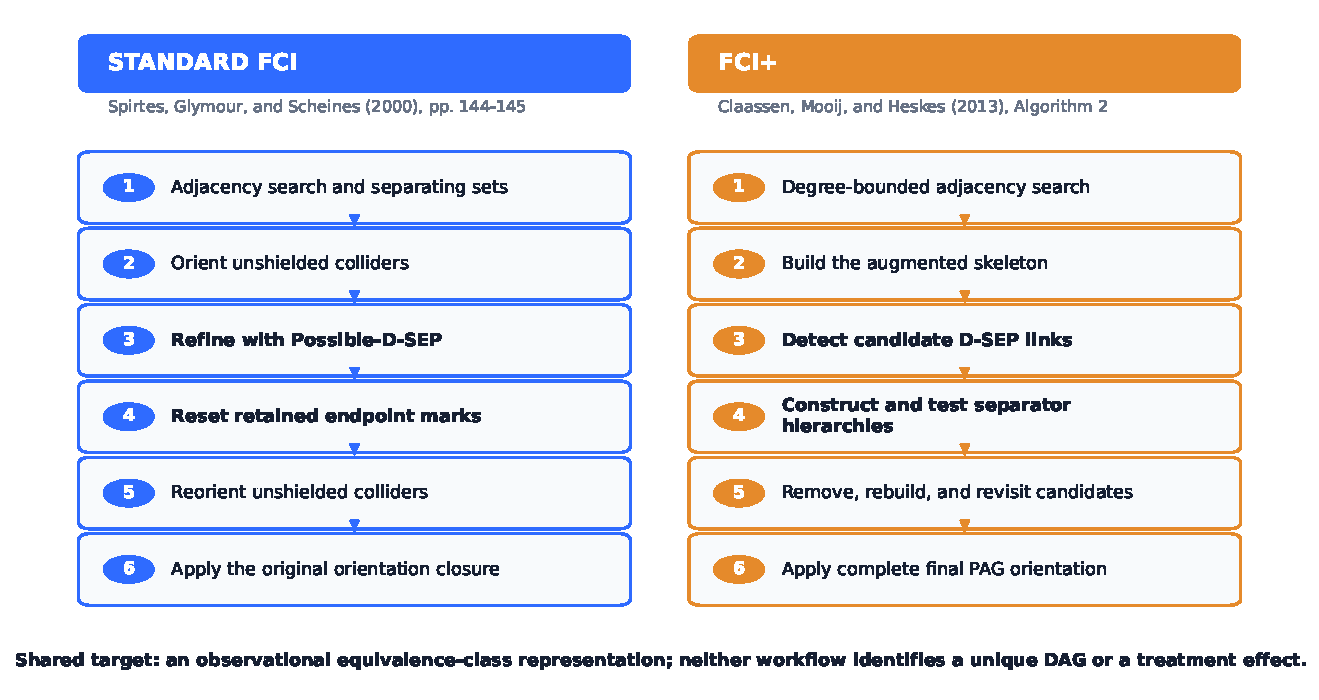
\includegraphics[width=\textwidth]{fci_fci_plus_workflow.pdf}
\caption{Source-located control-flow comparison. Standard FCI performs a
non-local Possible-D-SEP refinement; \FCIplus{} instead iterates
augmented-skeleton, candidate D-sep-link, hierarchy, and minimal-separator
stages before invoking final orientation. The robust application profile of
\cref{sec:implementation} changes finite-sample policy, not the definition of
Algorithm~2.}
\label{fig:workflow}
\end{figure}

\subsection{What the sources do not establish}

Neither source guarantees finite-sample recovery: both theorems are conditional
on correct CI decisions, and no bound is given for Fisher-Z, G-square, kernel,
or missing-data tests at a given \(N\). Neither identifies a unique DAG, an
adjustment set, or a treatment effect; a bidirected endpoint pattern does not
name, count, or measure a hidden cause. The 2000 source proves no maximal
orientation and gives no fixed-degree polynomial bound. The 2013 source proves
no finite-sample superiority over standard FCI, no wall-clock dominance, and no
guarantee when \(k\) is wrong or growing; a user-entered sparsity bound is not
evidence that the assumption holds. \citet{claassen2013learning} also warn that
hierarchy-derived conditioning sets may be large and may reduce finite-sample
power.

\section{Independent Python Implementation}
\label{sec:implementation}

\subsection{Package boundary and public API}

The objective is not to relabel a generic constraint-based search as
\FCIplus{}, but to expose the algorithmic obligations of \cref{sec:sources} as
inspectable components and keep them separate from finite-sample application
policy. Reusable code resides in \code{src/fci\_engine}; the STAR workflow
resides in \code{case\_studies/tennessee\_star}. No STAR variable, temporal
constraint, discretisation choice, or substantive conclusion is embedded in the
estimator package.

The top-level functions keep the two algorithms as separate entry points, and
paper profiles are explicit because a default optimised for finite samples
should not silently stand in for the source algorithm. \code{FCIConfig.paper()}
fixes unbounded depth and path length, immediate skeleton deletion, first-found
separators, enabled Possible-D-SEP, nonconservative colliders, and the
historical \code{spirtes\_2000} orientation closure. \code{FCIPlusConfig.paper(k)}
requires an explicit \(k\), assigns it to both the initial conditioning depth
and the endpoint-base sparsity bound, disables ordinary Possible-D-SEP, uses
immediate deletion and first-found separators, and selects the complete
\code{standard} orientation schedule required by Algorithm~2's output claim.
Profiles constrain execution; they do not validate theorem assumptions.
Supplying \(k=3\) does not prove that the unknown true MAG has degree at most
three.

The \code{PAG} class stores an endpoint mark at each side of every adjacency
while exposing the adjacency once, so tails, arrowheads, circles, and absence
are represented explicitly rather than flattened into a directed graph.
Mutations validate both nodes and reject one-sided or \code{NONE}-marked edges.
Every search uses one \code{CITest.test(data, x, y, cond\_set)} contract, with
built-in Fisher-Z, missing-value Fisher-Z, chi-square, G-square, and kernel CI
tests. A cache canonicalises the unordered pair and conditioning set, so the
result separates the number of \emph{logical} CI requests made by control flow,
the subset answered from cache, and the underlying statistical outcomes. This
distinction matters when connecting measurements to the \FCIplus{} theorem,
which counts oracle queries rather than elapsed time.

\subsection{Pipelines, orientation strategies, and profiles}

\code{FCI.fit} exposes the source stage ordering directly: complete circle
graph and adjacency search; separator-based collider decisions; ordered
Possible-D-SEP refinement recording removals with source \code{pdsep}; endpoint
reset and collider reconstruction; then the configured closure.
\code{FCIPlus.fit} deliberately does not call Possible-D-SEP; it passes the
initial skeleton and separators to the Algorithm~2 search, which builds the
augmented skeleton, recognises literal bidirected witness patterns, enumerates
paired endpoint bases, expands each hierarchy seed to a fixed point, tests the
resulting conditioning set, minimises the separator, updates the graph with
source \code{fci\_plus\_dsep}, and rebuilds candidates. A diagnostics record
counts candidate sightings and revisits, hierarchy queries and cache hits,
duplicate conditioning-set skips, D-SEP-stage CI requests, removed edges, and
the maximum tested conditioning size. These counters make a run inspectable;
they are empirical accounting, not a mechanised proof of the asymptotic bound.

One dispatcher provides explicit orientation schedules, and the separation is
part of the scientific interface. \code{spirtes\_2000} is the original
arrowhead and discriminating-path closure used by the standard-FCI paper
profile, historically aligned but not claimed maximally informative.
\code{standard} is the modern complete schedule including later
tail-completion rules, the appropriate completeness dependency for the
\FCIplus{} paper profile. \code{conservative} retains arrowhead conclusions
while suppressing tail-producing propagation; \code{leaf} permits a restricted
tail rule when the newly directed endpoint is a leaf; and \code{robust}
combines conservative collider decisions with the leaf-tail schedule. The last
three are finite-sample engineering policies and support no completed-PAG
claim. A dedicated regression verifies that the \code{spirtes\_2000} profile
stops before a selection-bias tail completion that \code{standard} can orient,
making the historical completeness boundary executable rather than merely
descriptive.

\begin{table}[H]
\caption{Published concept, repository symbol, and executable validation. A
``paper mechanism'' classification means the symbol implements the stated
source operation when invoked through the corresponding paper profile; it does
not mean the source proves every line of Python correct.}
\label{tab:traceability}
\footnotesize
\begin{tabularx}{\textwidth}{p{0.19\textwidth}p{0.295\textwidth}Yp{0.125\textwidth}}
\toprule
Published concept & Repository symbol & Principal validation &
Classification \\
\midrule
PC-style adjacency search &
\code{skeleton.\newline learn\_initial\_skeleton} &
skeleton, profile, and reference integration tests &
Shared \\
Possible-D-SEP criterion &
\code{pdsep.possible\_dsep} &
collider/triangle, tail blocking, cycles, path bounds &
Spirtes \\
Ordered Possible-D-SEP search &
\code{pdsep.\newline refine\_skeleton\_\newline with\_pdsep} &
both-direction and no-mixed-pool tests &
Spirtes \\
Original orientation closure &
\code{rules.\newline apply\_orientation\_rules}\newline (\code{spirtes\_2000}) &
orientation-rule tests; historical stopping regression &
2000-aligned, incomplete by source \\
Complete modern orientation &
\code{rules.\newline apply\_orientation\_rules}\newline (\code{standard}) &
\code{test\_oracle\_\newline pag\_rules.py} &
Later Zhang dependency \\
Augmented skeleton &
\code{dsep.\newline build\_augmented\_skeleton} &
single-node-dependence and existing-edge tests &
Claassen \\
Candidate D-sep pattern &
\code{dsep.\newline possible\_dsep\_links} &
witness, cross-path, arrowhead, circle-rejection tests &
Claassen \\
Recursive hierarchy &
\code{dsep.hierarchy} &
fixed-point and excluded-pair cache-key tests &
Claassen \\
Separator minimisation and revisit &
\code{dsep.minimal\_dsep};\newline refinement loop &
minimisation, removal, failed-candidate revisit tests &
Claassen \\
Exact m-separation oracle &
\code{simulation.\newline MAGOracleCITest} &
\code{test\_oracle\_graphs.py} &
Validation apparatus \\
Stable deletion, max-\(p\) separators &
\code{FCIPlusConfig.\newline practical} &
configuration, order, finite-sample benchmark tests &
Engineering extension \\
Structured trace and exports &
\code{result.FCIResult} &
\code{test\_result\_exports.py} &
Engineering extension \\
\bottomrule
\end{tabularx}
\normalsize
\end{table}

\code{FCIResult} binds the final graph to the evidence that produced it: the
resolved configuration, sample and node counts, separators and their stage
sources, logical CI count, cache hits, named CI and orientation traces,
ambiguous triples, D-SEP diagnostics, and elapsed time.
\code{explain\_edge(x,y)} returns the final marks, the separator and its
provenance when removed, all direct CI events for the pair, and the attached
orientation events; \code{save\_artifacts} exports JSON, a semantic endpoint
CSV, and standalone HTML. This prevents a plotted arrow from becoming detached
from the profile, CI test, threshold, or orientation decision that created it.
The package is typed and ships \code{py.typed}; the quality workflow runs
Pytest, Ruff, strict MyPy, wheel construction, installation, and an import
smoke test. Those checks establish interface and packaging consistency; they do
not validate faithfulness, true sparsity, CI-test model assumptions, or an
empirical causal conclusion.

The practical profile does not claim that uncertainty has been eliminated.
Stable deletion reduces one source of variable-order dependence; max-\(p\)
separator selection spends more CI queries to retain stronger sample
independence evidence at a fixed depth; conservative collider and tail policies
preserve circles where sample evidence is ambiguous; and automatic \(\alpha\)
is a documented sample-size heuristic. Each choice can improve a predefined
robustness metric while weakening informativeness or increasing computation.
Accordingly, ``paper \FCIplus{}'' is the fidelity and query-efficiency subject,
and ``robust \FCIplus{}'' is the preferred engineering policy for the reported
application because it meets the stated audit criteria while returning
less-specific endpoints. That preference is local to the evidence and criteria
in this project; it is not a universal accuracy ranking.

\subsection{Engineering scope}

\Cref{tab:scale} summarises the committed code base, all of it written for
this project. Line counts are raw file lengths including docstrings and blank
lines; the algorithm package alone contains 8,323 non-blank, non-comment
lines. The package exports 47 public symbols, ships \code{py.typed}, and
passes Ruff, strict MyPy, a wheel build, and an installed-import smoke test,
with Pytest executed independently on Python 3.9 through 3.13. Every number in
this report can be regenerated from the committed artifacts by the scripts in
the last row and \cref{sec:conclusions}.

\begin{table}[H]
\caption{Scale of the committed implementation and validation code.}
\label{tab:scale}
\small
\begin{tabularx}{\textwidth}{p{0.27\textwidth}Yr}
\toprule
Component & Contents & Lines \\
\midrule
Algorithm package \code{src/fci\_engine} &
38 typed modules: PAG endpoint algebra; five CI tests with canonical caching;
skeleton, Possible-D-SEP, and Algorithm~2 searches; orientation engine;
accuracy and stability metrics; MAG-oracle simulation; result and report
exports & 9,559 \\
\hspace{1em}of which \code{discovery/rules.py} &
complete arrowhead, discriminating-path, and R5--R10 tail rules under five
strategy schedules & 1,422 \\
Test suite \code{tests/} &
367 collected tests in 44 modules: unit, exact-oracle, property, integration,
typing, and report regressions & 5,929 \\
STAR application &
cohort coding, three-panel discovery suite, school-cluster bootstrap,
cyclic-order audit, standalone HTML report & 3,052 \\
Independent R reference &
\code{pcalg::fciPlus} runner with matched G-square semantics & 396 \\
Benchmarks, examples, and figure generators &
deterministic scripts behind every reported table and figure & 6,356 \\
\midrule
Total & & \(\approx\)25,300 \\
\bottomrule
\end{tabularx}
\end{table}

\section{Algorithm Validation}
\label{sec:validation}

\subsection{Exact oracle tests}

The strongest algorithm tests replace sample-based CI decisions with exact
m-separation in a known MAG, isolating graph-search correctness from sampling
error. The regression suite contains three independently specified targets
based on published structures: the canonical Figure~4(b) D-SEP example of
\citet{claassen2013learning}; a latent-variable reference graph derived from
the FCI literature; and an orientation-rule reference graph associated with the
completeness results of \citet{zhang2008completeness}. Both FCI and \FCIplus{}
recover the specified target PAGs on all three encoded fixtures, and
Figure~4(b) is additionally tested under four variable orders.

The Figure~4(b) MAG has the six edges \(Z \rightarrow U\), \(Z \rightarrow V\),
\(U \leftrightarrow X\), \(V \rightarrow X\), \(U \rightarrow Y\), and
\(V \leftrightarrow Y\). The adjacency stage retains a false \(X - Y\) link,
while \(X \perp Y \mid \{U,V,Z\}\) and \(Z\) is adjacent to neither endpoint.
The source exhibits this separator and identifies \(Z\) as the D-sep node; it
does not print an endpoint-complete PAG, so the completed comparison target is
repository derived and is described as such.

\begin{figure}[H]
\centering
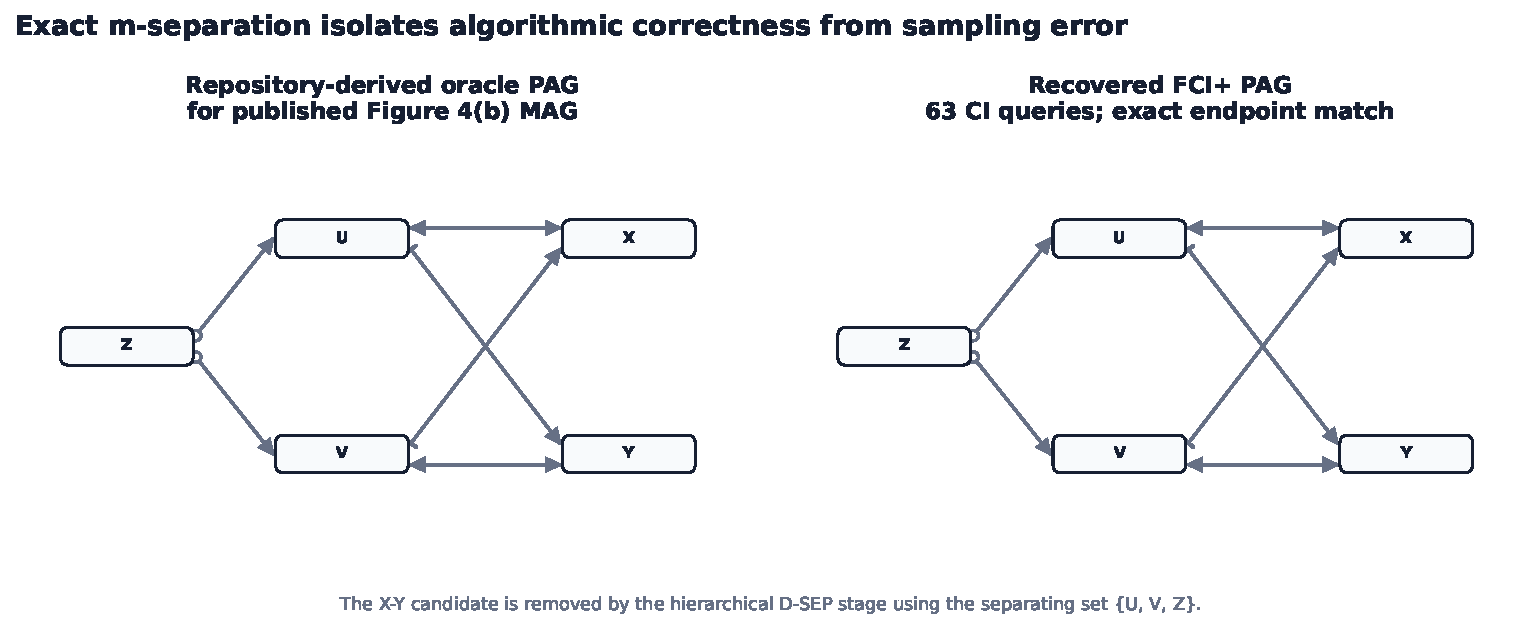
\includegraphics[width=\textwidth]{figure4_validation.pdf}
\caption{Exact-oracle validation on the central Figure~4(b) example. The
source-grounded facts are the six MAG edges and the exhibited separator; the
endpoint-complete comparison target is independently derived in the
repository.}
\label{fig:figure4}
\end{figure}

\begin{table}[H]
\caption{Paper-aligned Figure~4(b) oracle comparison.}
\label{tab:figure4-results}
\centering
\begin{tabular}{lrrl}
\toprule
Algorithm & CI queries & Difference & Final PAG \\
\midrule
Standard FCI & 102 & reference & Exact \\
\FCIplus{} & 63 & \(-39\) (\(-38.2\%\)) & Exact \\
\bottomrule
\end{tabular}
\end{table}

These values are frozen in \code{reports/data/oracle\_validation\_summary.csv}
together with the target PAG hash, the exact-oracle profile, query counts,
separator provenance, endpoint metrics, and execution status.

\subsection{Finite-sample behaviour}

Real data replace exact answers with noisy statistical decisions. A seeded
latent linear SEM based on the same reference graph gives an integration
result: at \(N = 5{,}000\), \FCIplus{} returns an extra \(X \leftrightarrow Y\)
with exact-edge F1 0.923 while standard FCI recovers the exact PAG, because the
sample CI decisions do not expose the \FCIplus{} D-SEP candidate; at
\(N = 50{,}000\) both recover the exact PAG. Logical query counts are 102 and
52 at \(N = 5{,}000\), and 102 and 63 at \(N = 50{,}000\), for FCI and
\FCIplus{} respectively. This is a reproducible fixture, not a universal
sample-size threshold.

The application safeguard was also tested on 15 deterministic latent-SEM cases:
five realistic graph families, three seeds each, 2,500 observations per case,
with a known oracle PAG.

\begin{table}[H]
\caption{Mean recovery across 15 finite-sample oracle cases.}
\label{tab:robust-finite-sample}
\centering
\begin{tabular}{lrrrrr}
\toprule
Profile & Skeleton F1 & Exact F1 & Semantic F1 & Endpoint acc. & CI calls \\
\midrule
Paper \FCIplus{} & 0.979 & 0.536 & 0.951 & 0.744 & 197.1 \\
Robust \FCIplus{} & 0.985 & 0.730 & 0.985 & 0.840 & 401.9 \\
\bottomrule
\end{tabular}
\end{table}

The robust profile improves the mean skeleton and endpoint-oriented scores on
these runs while using about 2.04 times as many CI calls. This does not prove
universal dominance, but it is a known-truth check that the STAR stability gain
is not obtained by simply discarding useful structure. It also warns against
assuming that fewer CI tests imply uniformly better finite-sample accuracy: FCI
and \FCIplus{} can make different errors because they take different logical
search routes after the initial skeleton.

\keyresult{The oracle tests support the correctness of the implemented FCI and
\FCIplus{} search-and-orientation pipeline under exact conditional-independence
information. The finite-sample tests simultaneously show that empirical results
remain limited by CI-test error and tuning choices.}

\section{Comparison with Established Software}
\label{sec:software}

The comparison separates execution from interface inspection. The executed
layer asks what happened on identical committed datasets under recorded
settings; the capability layer asks what each public interface or official
documentation exposes. Tetrad 7.6.10 appears only in the latter as a
documentation-only comparison, because no working Java runtime was available in
the recorded environment; no empirical row or runtime is attributed to it. All
claims are dated 26 July 2026.

The benchmark contains five realistic latent-SEM scenarios, three deterministic
repetitions each, and 2,500 observations per run, with every method receiving
the same numeric matrix and variable order. Fixed paper and reference rows use
Fisher-Z at \(\alpha = 0.001\); robust \FCIplus{} uses its documented
sample-size rule, which resolves to \(\alpha = 0.01\) here. The mismatch is
intentional because that row evaluates the public robust policy, not a literal
Algorithm~2 reproduction.

\begin{table}[H]
\caption{Executed known-truth comparison: means over 15 completed runs.}
\label{tab:executed-software-benchmark}
\begin{tabularx}{\textwidth}{p{0.235\textwidth}rrrrrY}
\toprule
Method (version) & Skeleton F1 & Exact F1 & Semantic F1 &
Endpoint acc. & Seconds & Logical CI \\
\midrule
Local FCI paper (0.1.0) & 0.977 & 0.532 & 0.943 & 0.737 & 0.020 & 449.7 \\
Local \FCIplus{} paper (0.1.0) & 0.979 & 0.536 & 0.951 & 0.744 & 0.009 & 197.1 \\
Local \FCIplus{} robust (0.1.0) & 0.985 & 0.730 & 0.985 & 0.840 & 0.018 & 401.9 \\
causal-learn FCI (0.1.4.7) & 0.979 & 0.536 & 0.951 & 0.744 & 0.009 & not exposed \\
\code{pcalg::fciPlus} (2.7-12) & 0.979 & 0.536 & 0.951 & 0.744 & 0.500 & not exposed \\
\bottomrule
\end{tabularx}
\end{table}

\begin{figure}[H]
\centering
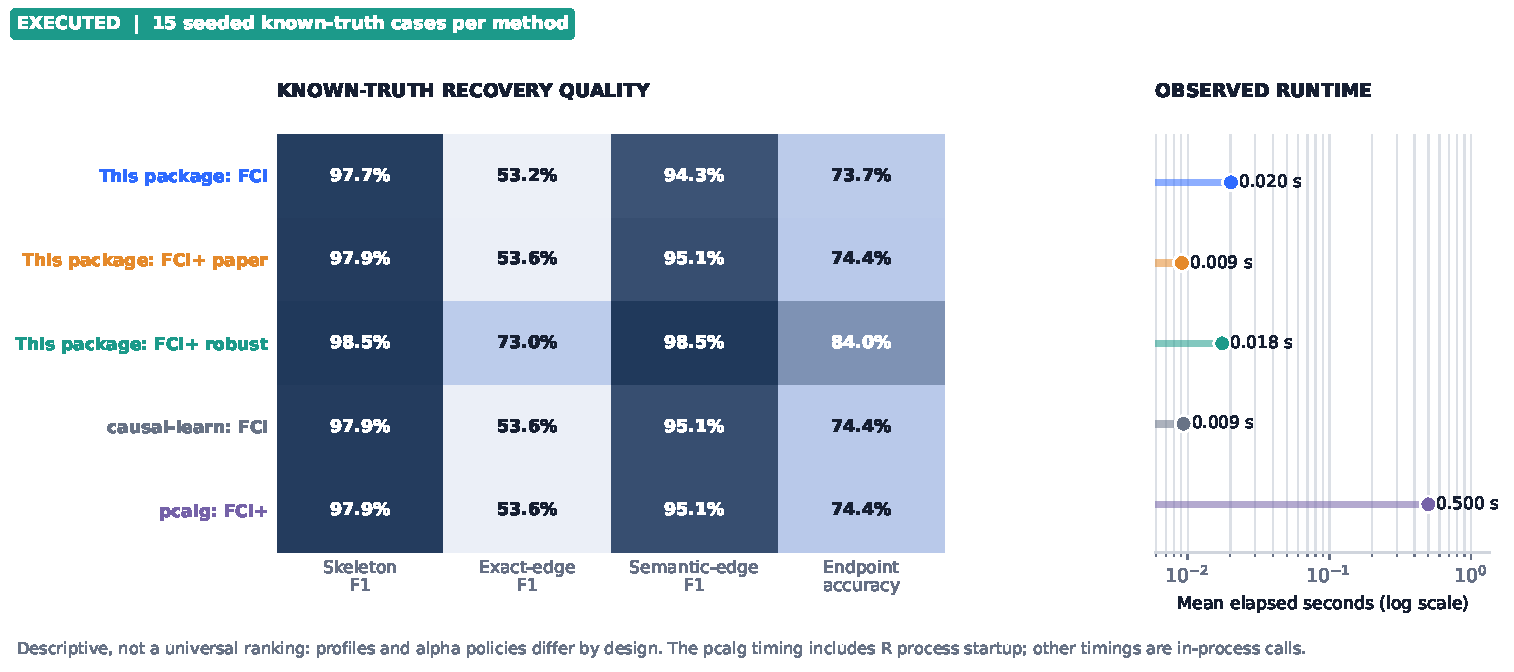
\includegraphics[width=\textwidth]{software_benchmark_comparison.pdf}
\caption{Matched known-truth comparison. The robust profile improves the
reported endpoint-oriented means on these scenarios while retaining a similar
skeleton score and spending more logical CI queries than paper \FCIplus{}.}
\label{fig:software-benchmark}
\end{figure}

Exact F1 requires both endpoint marks to match; semantic F1 additionally
credits endpoint patterns compatible with the target ancestral constraints;
endpoint accuracy scores individual marks. The common conversion represents
each PAG edge as an unordered node pair plus two semantic marks and never
interprets raw package matrices as generic directed edges. The equality of the
aggregate local paper-\FCIplus{}, causal-learn, and \code{pcalg} scores is
useful differential evidence on these fixtures, not an equivalence proof: local
and causal-learn times cover in-process calls whereas the R timing includes
process startup, and \code{pcalg::fciPlus} does not expose an identical control
for the true-degree bound \(k\).

Every comparison obeys five rules. Circles, tails, and arrowheads are preserved
in semantic normalisation. Data, order, alpha, CI semantics, and search caps are
held fixed where interfaces allow, and every mismatch is disclosed. Standard
FCI, Claassen \FCIplus{}, and other FCI-family hybrids are not relabelled as one
algorithm. Logical queries, cache hits, executed statistical tests, and wall
time remain different quantities. Smoke-call success establishes callability,
not scientific validity. On the capability layer, \code{pcalg} exposes both FCI
and \FCIplus{} and accepts user-defined CI tests, and its standard-FCI result
exposes separator information, but its inspected \code{fciPlus} result carries
materially less separator provenance; causal-learn exposes standard FCI and
named CI methods but no inspected public Claassen \FCIplus{} entry point; Tetrad
provides FCI and several FCI-family or hybrid searches, none of which was
established as a drop-in Claassen \FCIplus{}.

\keyresult{The local package integrates paper-profile control, structured CI
and orientation traces, separator-source provenance, D-SEP diagnostics,
per-edge explanations, stability auditing, and bundled artifacts in one Python
workflow, which was not found as a single public workflow in the checked
interfaces. This is an auditability and integration improvement, not a
universal accuracy or speed superiority claim.}

\section{STAR Study Design and Methods}
\label{sec:star-design}

\subsection{Experiment, cohort, and panels}

The Tennessee Student/Teacher Achievement Ratio project was a large randomized
experiment in kindergarten through grade 3, assigning students and teachers to
small classes, regular classes, or regular classes with a full-time aide;
official documentation describes small classes of approximately 13--17 students
and regular classes of approximately 22--25 \citep{word1990star}. Subsequent
economic analysis has used STAR as a central source of evidence on class size
\citep{krueger1999experimental}. This analysis uses the official Harvard
Dataverse release \citep{achilles2008star}: 11,601 student records, 379
variables, CC0 1.0, with codes checked against the accompanying 146-page user
guide.

Randomization already provides a stronger basis for estimating the class-size
effect than an unconstrained structure-learning algorithm, so FCI is not used to
rediscover it. The purpose is to examine whether grade-3 observation is
structurally related to early achievement or background variables; whether early
and later achievement remain adjacent after conditioning on measured context;
how the learned PAG changes when an early post-assignment outcome is included or
excluded; whether FCI and \FCIplus{} agree on skeletons and important
adjacencies; and how much search work \FCIplus{} saves on real data. The design
also supplies an unusually useful external audit: if a data-only PAG implies an
implausible pre-treatment direction, or suggests latent confounding of a
genuinely randomized assignment, the discrepancy should be reported rather than
accepted literally.

The analysis begins with the 6,325 students who have a kindergarten class
assignment, across 79 kindergarten schools, and builds three panels that are
deliberately not pooled because each encodes a different statistical question.

\begin{table}[H]
\caption{STAR analysis panels.}
\label{tab:panels}
\begin{tabularx}{\textwidth}{lrrY}
\toprule
Panel & Rows & Nodes & Purpose \\
\midrule
Attrition / observation & 5,744 & 9 &
Relate assignment, characteristics, context, and kindergarten achievement to
whether both grade-3 scores are observed. \\
Longitudinal achievement & 2,787 & 9 &
Study structure between kindergarten and grade-3 achievement among complete
cases while retaining early achievement. \\
Focused treatment-outcome & 2,976 & 8 &
Study the class-assignment/grade-3 relationship without allowing kindergarten
achievement, an early post-assignment outcome, to serve as a separator. \\
\bottomrule
\end{tabularx}
\end{table}

All model inputs are integer-coded discrete categories: class arm, sex,
ethnicity (with smaller source categories collapsed to \emph{Other} to avoid
extremely sparse contingency cells), free-lunch status, school context, entry
age in quantile categories, binned teacher experience, and reading-plus-mathematics
scaled scores converted to achievement quartiles. The exact numeric tables
supplied to the algorithms are committed under
\code{case\_studies/tennessee\_star/data/processed}.

\subsection{Analysis protocol}

Before discovery, the report computes observed means and randomized-arm
contrasts for the kindergarten score sum, the grade-3 score sum among students
with both scores, and the probability that both grade-3 scores are observed,
with uncertainty from 1,000 bootstrap samples of kindergarten schools.
Resampling schools rather than students preserves the main within-school
dependence. These contrasts are reported separately from FCI output because
they use the experiment's assignment as the basis for interpretation.

Discovery uses the likelihood-ratio G-square test,
\(G^2 = 2 \sum_s \sum_{x,y} O_{xys} \log ( O_{xys} / E_{xys} )\), with
zero-count contributions omitted. The test suits the discretised panels, but
high-order conditioning can create sparse cells.

\begin{table}[H]
\caption{Primary STAR discovery configuration.}
\label{tab:star-config}
\begin{tabularx}{\textwidth}{lY}
\toprule
Setting & Value \\
\midrule
CI test & G-square on discretised variables \\
Significance threshold & \(\alpha = 0.05\) \\
Standard FCI & \code{profile="paper"}; unbounded paper schedule \\
Paper \FCIplus{} & \code{profile="paper"}; \(k = 3\) \\
Robust application \FCIplus{} & \code{profile="practical"}; stable skeleton;
strongest separating set; conservative colliders; robust orientation; depth and
sparsity bound 3 \\
R reference & \code{pcalg::fciPlus}; selection bias enabled; no exposed
explicit \(k\) \\
Timing & Three full-data repetitions; median elapsed time reported \\
PAG stability & 100 kindergarten-school cluster bootstrap fits per algorithm
and panel \\
Order audit & Every cyclic column shift for all local profiles and the R
reference \\
Prior temporal constraints & None supplied to discovery; temporal reversals are
audited after fitting \\
\bottomrule
\end{tabularx}
\end{table}

For stability, the 79 schools are sampled with replacement, all student rows
from a selected school are included, the algorithm is refitted, and each
unordered adjacency is recorded; with \(B = 100\) replicates the estimated
frequency is \(\hat{\pi}_{XY} = B^{-1}\sum_b \mathbf{1}\{X, Y \text{ adjacent in
replicate } b\}\). This is an exploratory stability diagnostic with
one-percentage-point resolution, not a confidence interval, a posterior edge
probability, or an endpoint-compatible uncertainty summary. The focused analysis
is additionally repeated for \(\alpha \in \{0.01, 0.05\}\), three versus four
quantile bins, and \FCIplus{} bounds \(k \in \{2,3,4\}\).

The application distinguishes a reproducible adjacency from a credible
direction. A skeleton-level conclusion is promoted only when the target
adjacency survives every cyclic column shift and has high bootstrap frequency. A
directional conclusion additionally requires invariant endpoint marks, no
conflict with measurement time or randomization, and no material reversal under
the sensitivity checks. Failure of the directional rule does not delete the
edge; it downgrades the claim to conditional-dependence structure with
unresolved direction.

\section{STAR Results}
\label{sec:star-results}

\subsection{Observed randomized-arm outcomes}

\begin{table}[H]
\caption{Observed outcome summaries by kindergarten class arm. Intervals use
1,000 kindergarten-school bootstrap samples.}
\label{tab:arm-summary}
\centering
\begin{threeparttable}
\begin{tabular}{llrrr}
\toprule
Outcome & Arm & \(n\) & Estimate & 95\% interval \\
\midrule
\multirow{3}{*}{Kindergarten score}
 & Regular & 2,005 & 918.04 & 908.78 to 927.05 \\
 & Regular + aide & 2,043 & 918.36 & 908.52 to 927.07 \\
 & Small & 1,738 & 931.94 & 922.70 to 940.12 \\
\addlinespace
\multirow{3}{*}{Grade-3 score}
 & Regular & 1,047 & 1246.74 & 1238.96 to 1254.01 \\
 & Regular + aide & 1,019 & 1247.25 & 1238.53 to 1255.48 \\
 & Small & 936 & 1258.43 & 1250.58 to 1266.17 \\
\addlinespace
\multirow{3}{*}{Grade-3 observed}
 & Regular & 2,194 & 47.72\% & 42.72\% to 52.14\% \\
 & Regular + aide & 2,231 & 45.67\% & 40.64\% to 50.39\% \\
 & Small & 1,900 & 49.26\% & 44.46\% to 53.77\% \\
\bottomrule
\end{tabular}
\begin{tablenotes}[flushleft]\small
\item Grade-3 summaries condition on both scores being observed. Kindergarten
summaries also exclude missing score components, so both are design-supported
observed-outcome comparisons rather than a fully reconstructed
intention-to-treat estimand.
\end{tablenotes}
\end{threeparttable}
\end{table}

\begin{figure}[H]
\centering
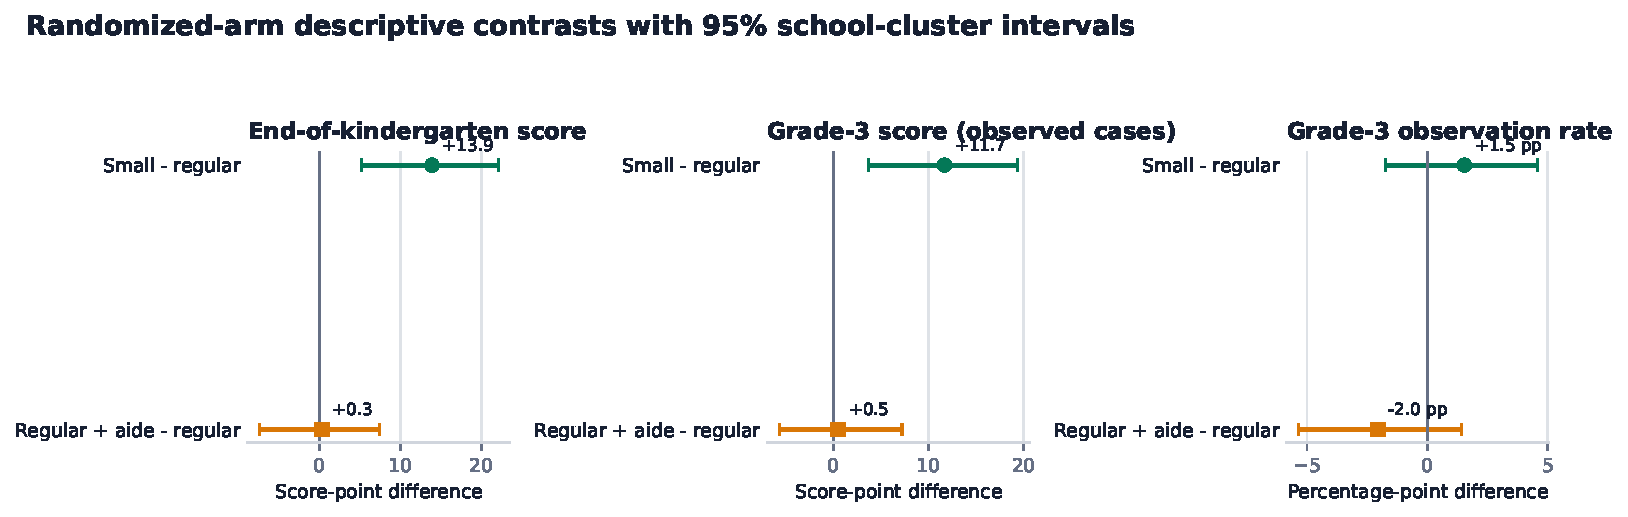
\includegraphics[width=\textwidth]{star_descriptive_contrasts.pdf}
\caption{Contrasts against the regular-class arm. Small classes show positive
score differences at kindergarten and grade 3 among observed cases; the aide arm
remains close to zero.}
\label{fig:contrasts}
\end{figure}

The small-minus-regular kindergarten contrast is 13.90 points, with a 95\%
school-cluster interval from 5.21 to 22.07, while the regular-with-aide contrast
is 0.31 points (\(-7.40\) to 7.38). At grade 3 among observed students the
small-class contrast remains positive at 11.69 points (3.74 to 19.38) and the
aide contrast is 0.51 points (\(-5.70\) to 7.22). Observation rates show no
precise arm difference: small minus regular is \(+1.54\) percentage points
(\(-1.73\) to 4.56) and aide minus regular is \(-2.05\) points (\(-5.35\) to
1.41).

\subsection{Attrition and longitudinal panels}

\begin{figure}[H]
\centering
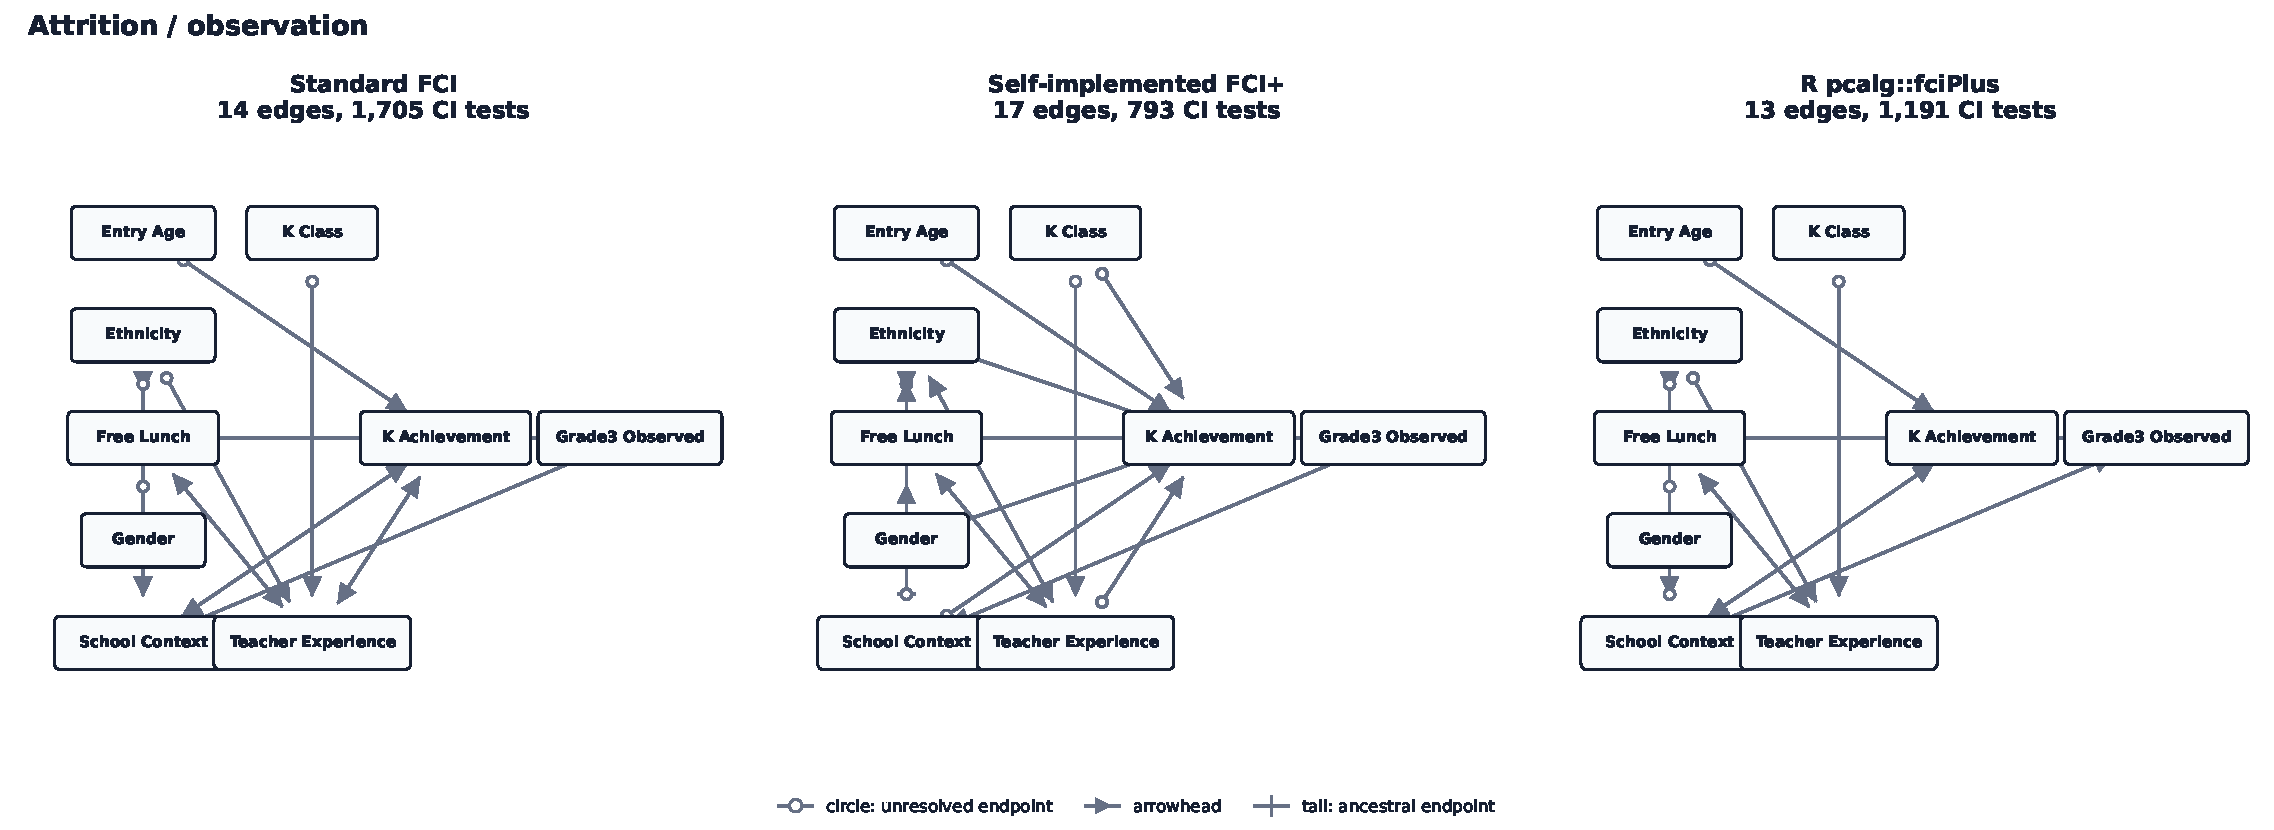
\includegraphics[width=\textwidth]{pag_attrition.pdf}
\caption{Three PAGs for the attrition/observation panel: self-implemented FCI,
self-implemented \FCIplus{}, and R \code{pcalg::fciPlus}. The skeletons
substantially overlap, while the achievement/observation endpoint differs.}
\label{fig:pag-attrition}
\end{figure}

On the attrition panel, standard FCI returns 14 edges after 1,705 CI tests,
self-implemented \FCIplus{} 17 edges after 793 tests, and R
\code{pcalg::fciPlus} 13 edges after 1,191 tests; pairwise skeleton Jaccard
values are 0.824, 0.929, and 0.765. All three omit a direct
\code{K\_Class}--\code{Grade3\_Observed} adjacency, which appears in only
12--16\% of the school bootstraps across local profiles. By contrast,
\code{K\_Achievement}--\code{Grade3\_Observed} is adjacent in 100\% of bootstrap
fits for all three local profiles, and the free-lunch/observation adjacency is
also stable. Later data availability is therefore not independent of early
achievement and measured socioeconomic or school context. The three endpoint
readings are revealing: standard FCI gives the impossible \emph{grade-3
observation \(\rightarrow\) kindergarten achievement}; self-\FCIplus{} leaves a
circle at the later endpoint; and R-\FCIplus{} gives the temporally admissible
direction. The R result is more plausible on this edge, but package identity
alone cannot establish that its orientation is statistically correct.

\begin{figure}[H]
\centering
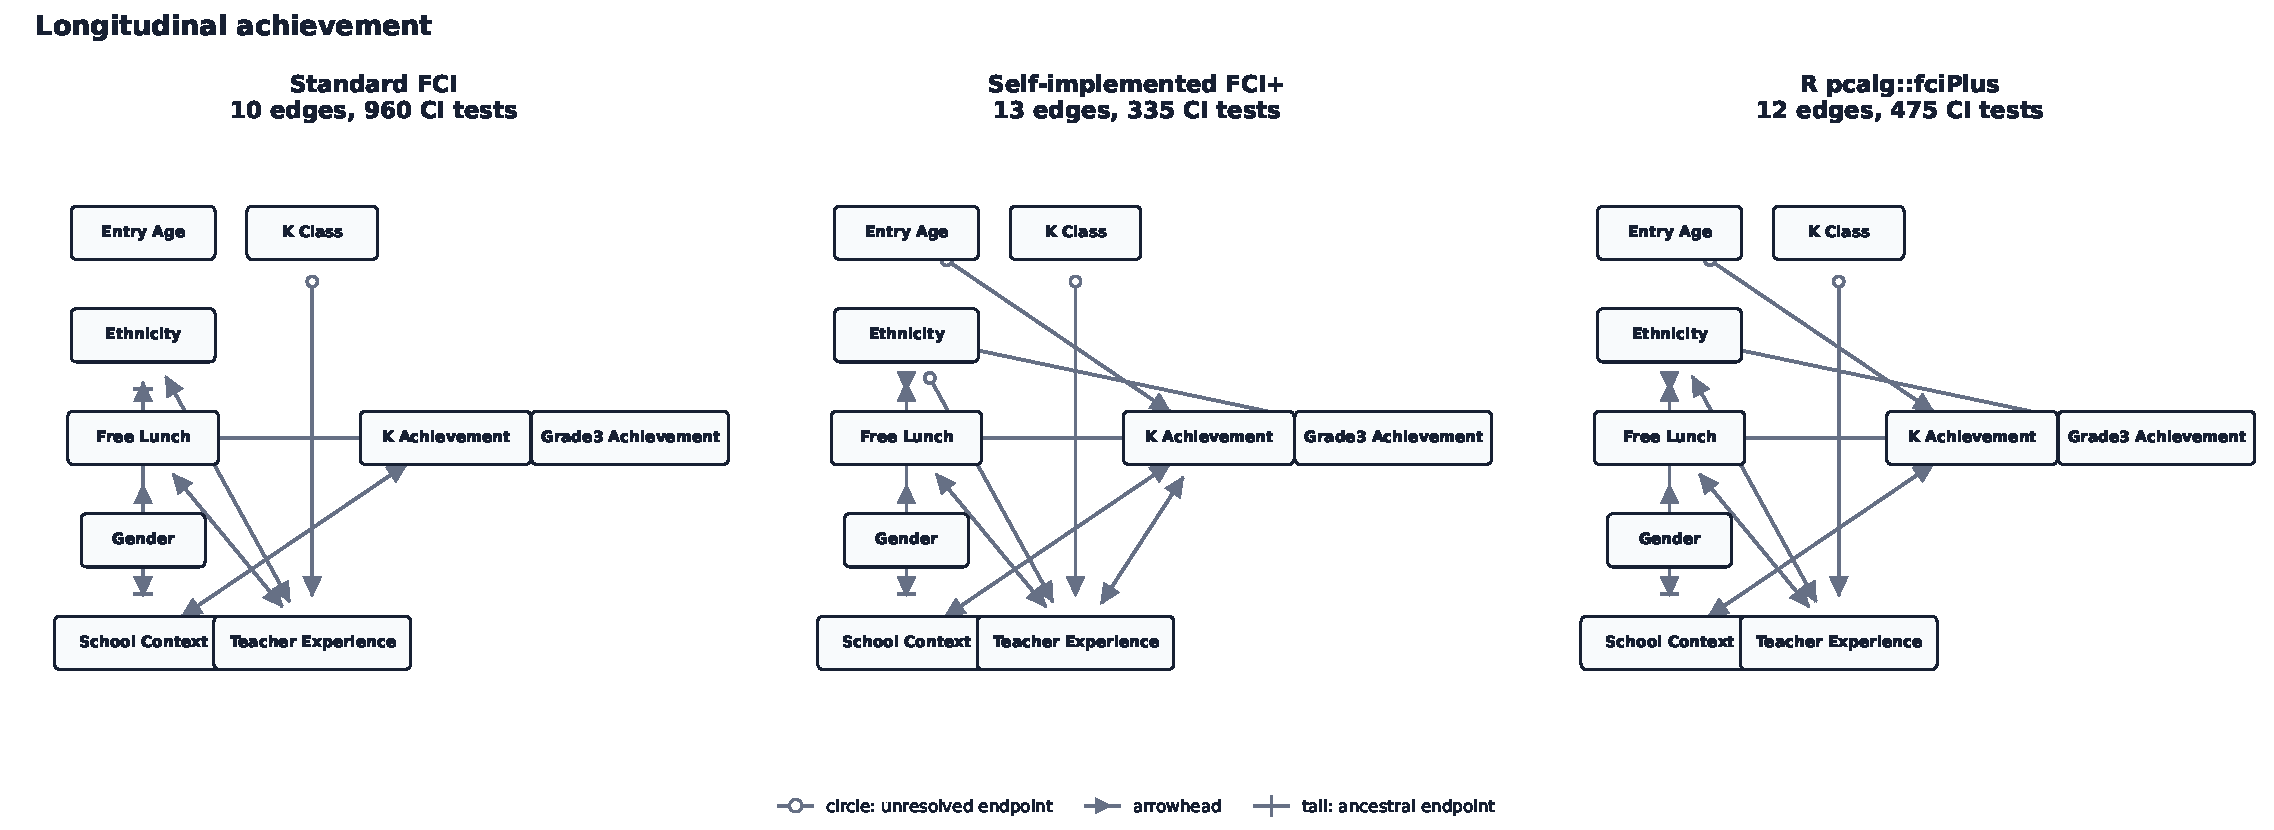
\includegraphics[width=\textwidth]{pag_longitudinal.pdf}
\caption{Three PAGs for the longitudinal complete-case panel. All retain the
kindergarten/grade-3 achievement adjacency, but both \FCIplus{} implementations
orient it against chronology.}
\label{fig:pag-longitudinal}
\end{figure}

On the longitudinal panel, standard FCI returns 10 edges and 960 tests,
self-\FCIplus{} 13 edges and 335 tests, and R-\FCIplus{} 12 edges and 475 tests,
with skeleton Jaccard 0.769, 0.833, and 0.923. All three retain the
kindergarten/grade-3 achievement adjacency, which appears in all 100 bootstrap
samples for all three local profiles. Neither full-data PAG retains a direct
class-assignment/grade-3 adjacency once kindergarten achievement is included,
yet that adjacency reappears in 71\% of FCI, 79\% of paper \FCIplus{}, and 80\%
of robust-profile bootstrap fits --- a warning that conservative orientation and
order invariance do not remove school-resampling sensitivity. Both \FCIplus{}
implementations orient grade-3 achievement toward kindergarten achievement,
which is temporally impossible if read causally, while standard FCI leaves that
endpoint unresolved. Agreement between two implementations is therefore not
sufficient to override chronology: they may replicate the same finite-sample CI
pattern and orientation logic under complete-case selection.

\cautionbox{The attrition PAG does not prove a particular missingness
mechanism. It shows that the observed conditional-independence structure links
grade-3 availability to earlier achievement and context. A formal missing-data
analysis would require an explicit estimand and additional assumptions.}

\subsection{Focused treatment-outcome panel}

\begin{figure}[H]
\centering
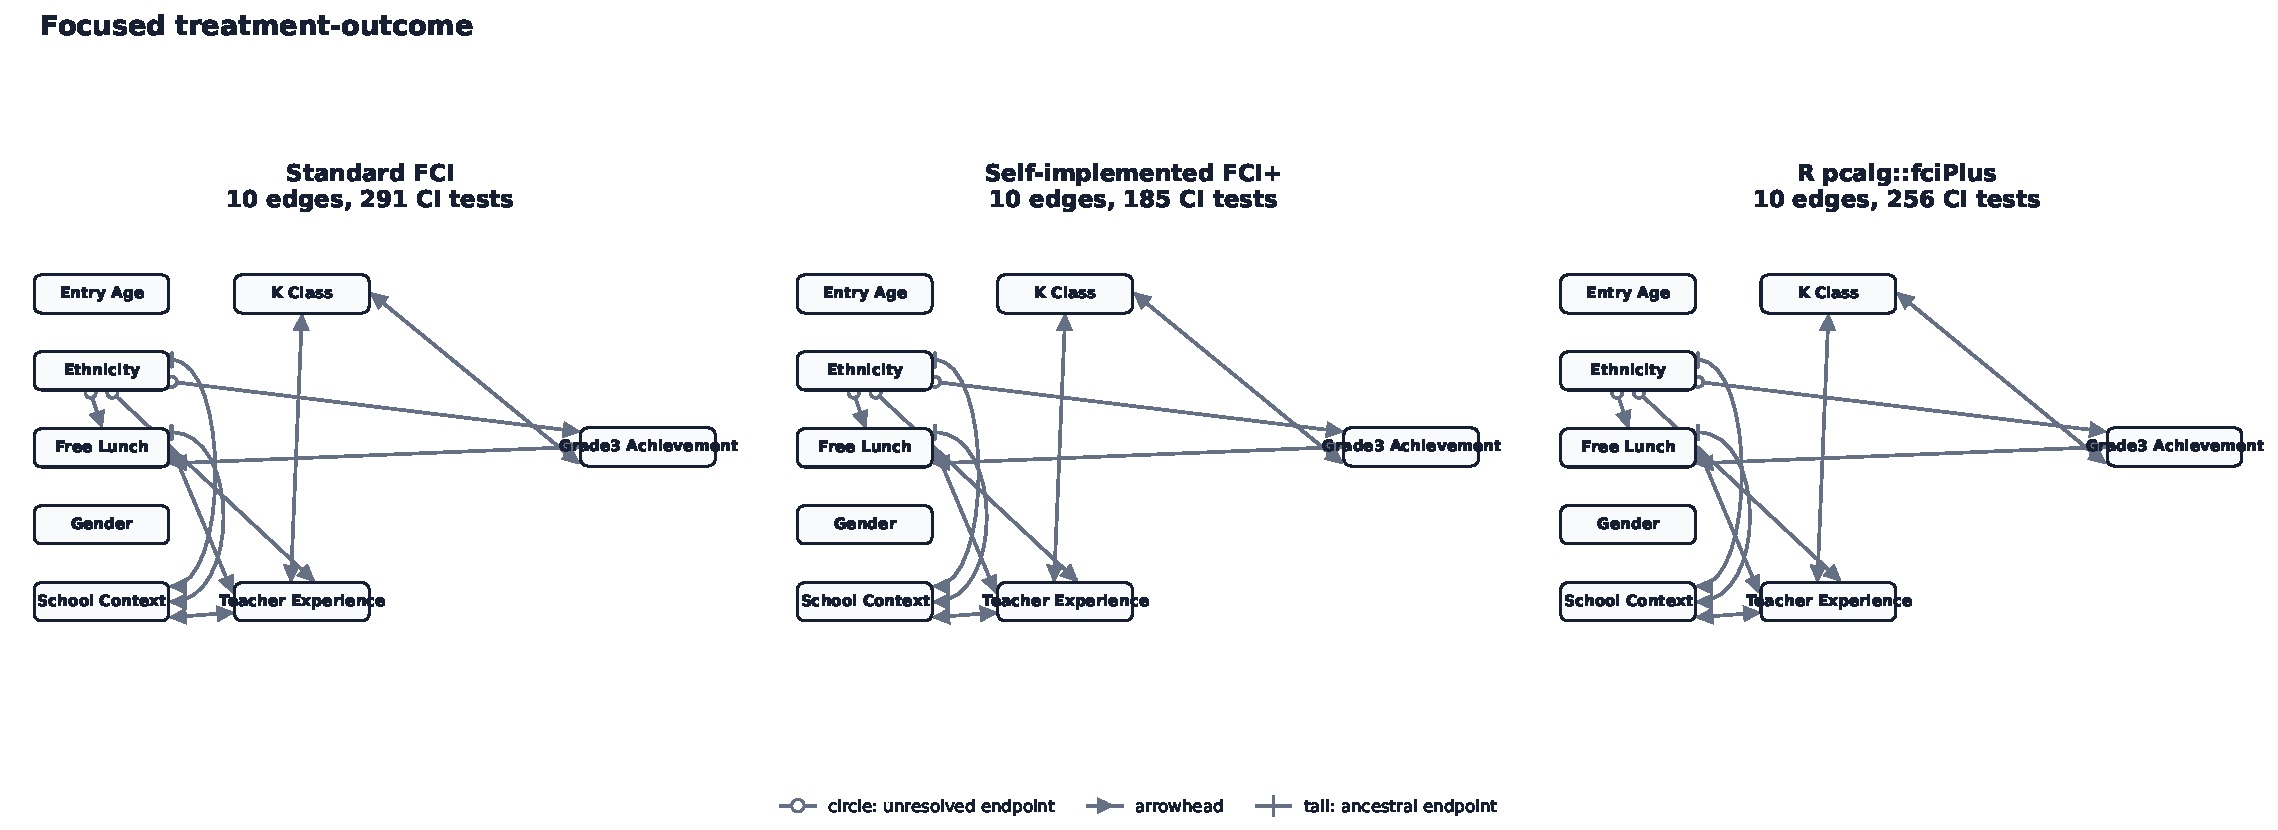
\includegraphics[width=\textwidth]{pag_focused_treatment.pdf}
\caption{PAGs for the focused complete-case panel. All three algorithms recover
the exact same 10-edge skeleton and endpoint pattern, including the bidirected
class-assignment/grade-3 edge.}
\label{fig:pag-focused}
\end{figure}

Removing kindergarten achievement from the node set changes the result.
Standard FCI, self-\FCIplus{}, and R-\FCIplus{} all return the same 10-edge PAG
--- not merely the same skeleton --- and all three contain
\(\mathit{K\_Class} \leftrightarrow \mathit{Grade3\_Achievement}\). The
adjacency appears in 92\% of FCI, 85\% of paper self-\FCIplus{}, and 96\% of
robust-profile bootstraps. Independent exact replication makes this observed
conditional-independence pattern more credible, but it does not make a literal
latent-confounding reading credible: kindergarten class assignment was
randomized, while the focused panel conditions on grade-3 outcomes being
observed and omits early post-assignment achievement. Conditioning on
observation, school-level dependence, omitted post-randomization variables, and
CI-test approximation can all create an observed pattern represented by
arrowheads at both endpoints.

\begin{figure}[H]
\centering
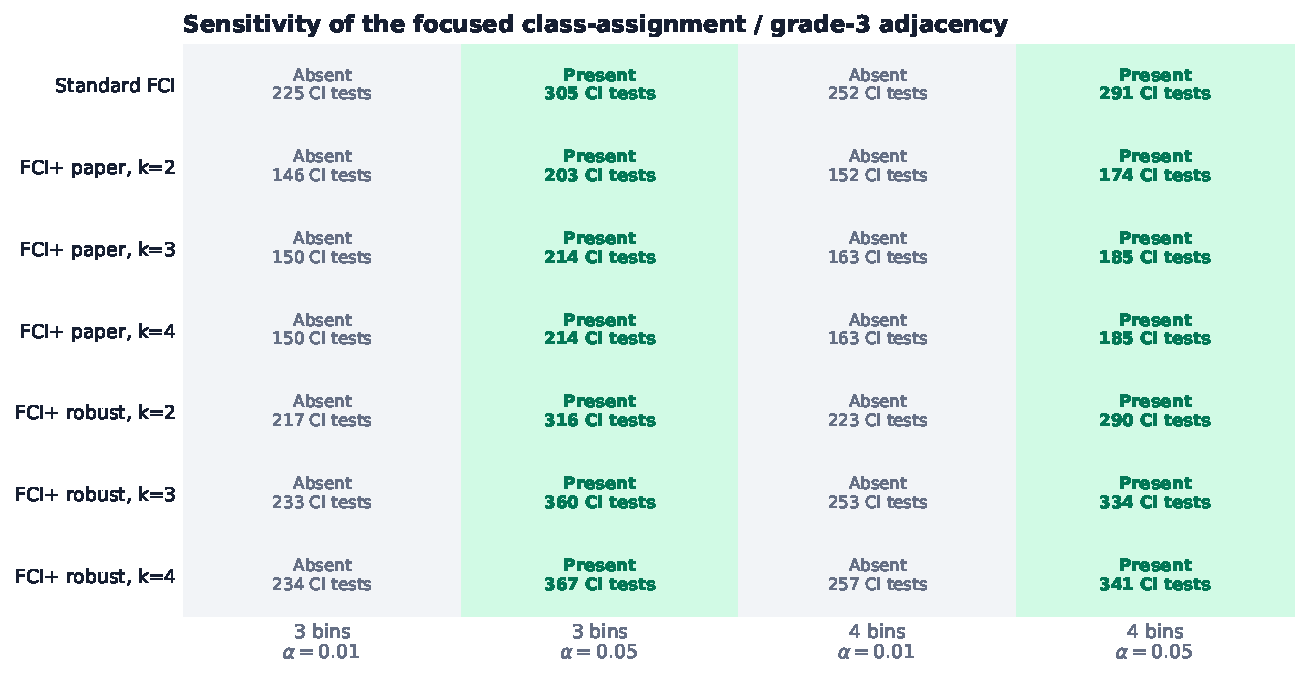
\includegraphics[width=0.92\textwidth]{star_sensitivity.pdf}
\caption{Focused treatment-outcome sensitivity. The adjacency appears at
\(\alpha = 0.05\) and disappears at \(\alpha = 0.01\), regardless of whether
three or four quantile bins or \(k = 2, 3, 4\) is used for \FCIplus{}.}
\label{fig:sensitivity}
\end{figure}

The sensitivity result is decisive for interpretation. The focused adjacency is
robust to the tested bin count and degree bound but not to the CI threshold: at
\(\alpha = 0.01\) no local configuration retains it, while at
\(\alpha = 0.05\) the paper profiles retain a bidirected mark for every tested
\(k\), and the robust endpoint is
\(\mathit{K\_Class} \leftarrow\!\circ\; \mathit{Grade3\_Achievement}\) with
three bins and \(\mathit{K\_Class} \circ\!-\!\circ \mathit{Grade3\_Achievement}\)
with four. The stricter threshold requires more evidence against conditional
independence before an edge is kept, so its removal indicates that the edge
rests on relatively weak conditional-dependence evidence rather than an
invariant feature across reasonable settings.

\subsection{Robust application profile, agreement, and cost}

\begin{figure}[H]
\centering
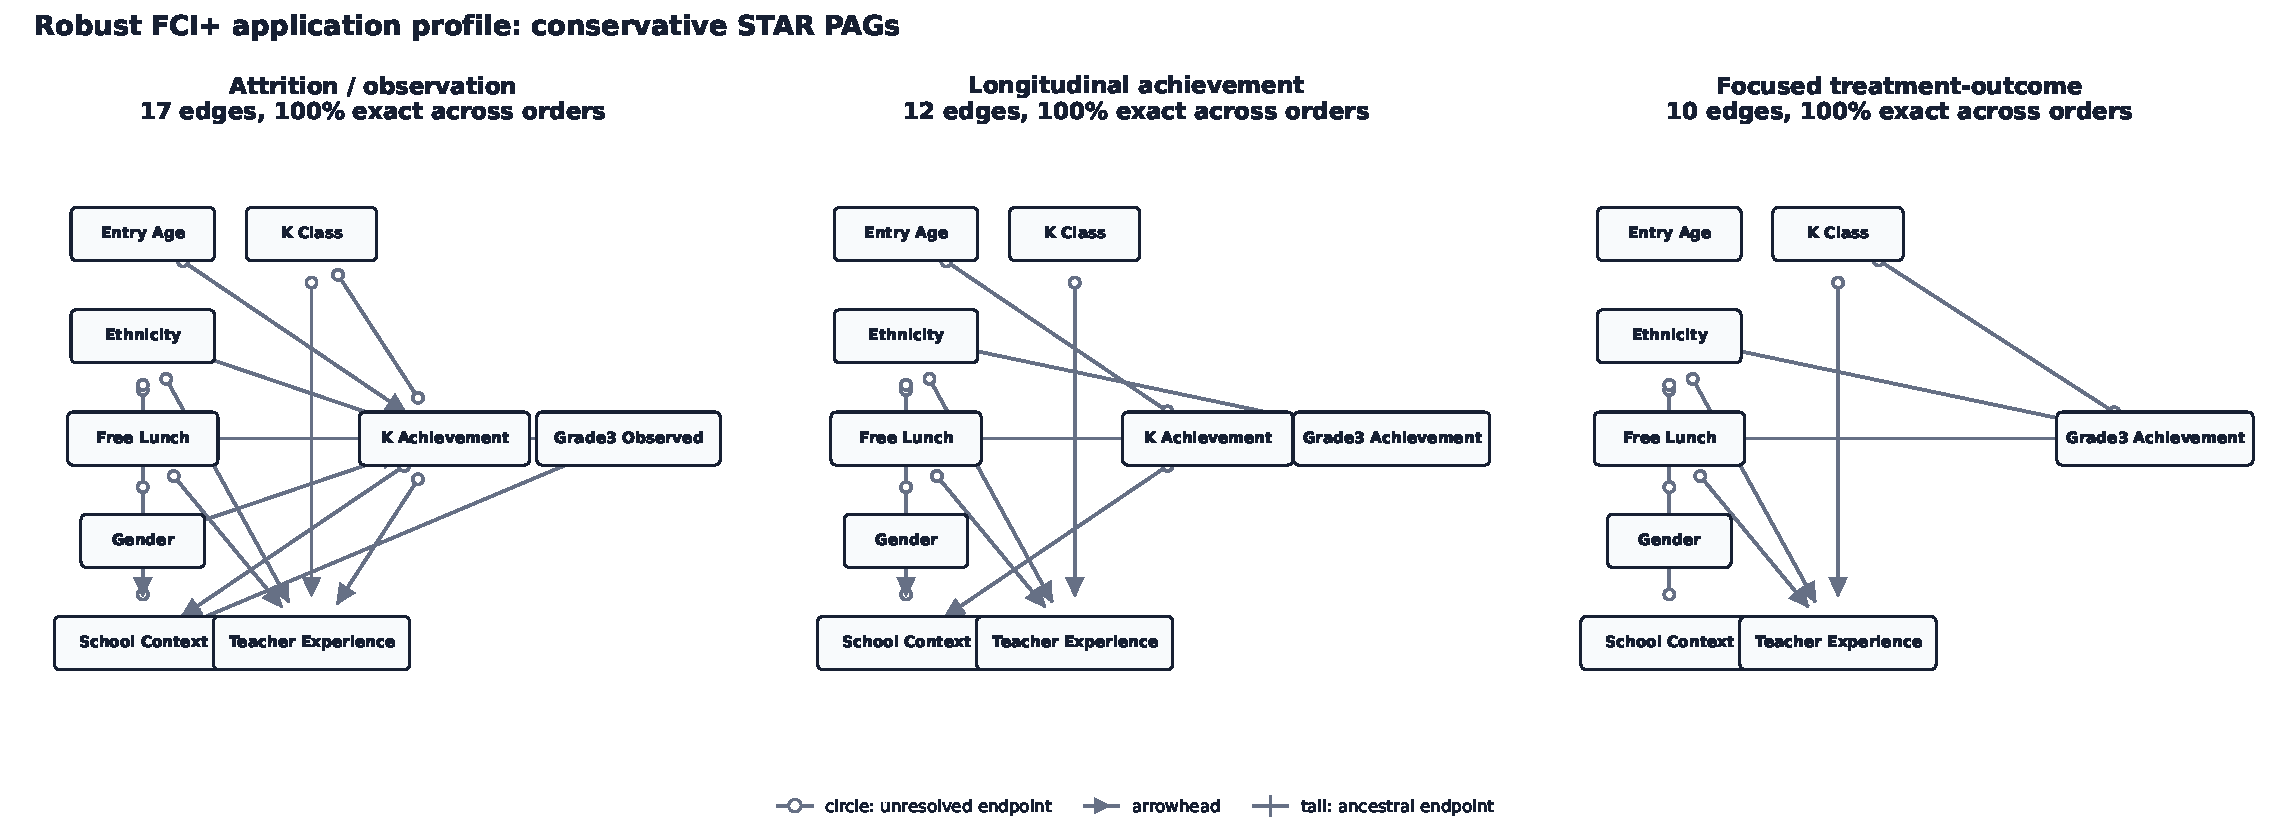
\includegraphics[width=\textwidth]{pag_robust_application.pdf}
\caption{The three STAR PAGs from the separate robust application profile.
Stable skeleton search and conservative orientation preserve the main
adjacencies while leaving unsupported directions unresolved.}
\label{fig:pag-robust}
\end{figure}

The robust profile is not a fourth paper implementation; it is a finite-sample
decision layer applied after the literal comparisons. It returns 17, 12, and 10
edges on the attrition, longitudinal, and focused panels, with target relations
\(\mathit{K\_Achievement} \circ\!-\!\circ \mathit{Grade3\_Observed}\),
\(\mathit{K\_Achievement} \circ\!-\!\circ \mathit{Grade3\_Achievement}\), and
\(\mathit{K\_Class} \circ\!-\!\circ \mathit{Grade3\_Achievement}\). It thus
retains the relevant skeleton information without repeating the paper-profile
chronology reversal or the focused-panel bidirected over-interpretation.

\begin{table}[H]
\caption{Cyclic-order audit for paper and robust self-\FCIplus{} profiles.}
\label{tab:robust-order-audit}
\centering
\begin{tabular}{llrrr}
\toprule
Panel & Profile & Exact PAG & Worst skeleton & Temporal reversals \\
\midrule
\multirow{2}{*}{Attrition} & Paper & 100.0\% & 100.0\% & 0 \\
 & Robust & 100.0\% & 100.0\% & 0 \\
\addlinespace
\multirow{2}{*}{Longitudinal} & Paper & 55.6\% & 92.3\% & 1 \\
 & Robust & 100.0\% & 100.0\% & 0 \\
\addlinespace
\multirow{2}{*}{Focused} & Paper & 75.0\% & 100.0\% & 0 \\
 & Robust & 100.0\% & 100.0\% & 0 \\
\bottomrule
\end{tabular}
\end{table}

The order audit rotates the input variable list through every cyclic shift. The
R reference preserves every panel skeleton while reproducing exact PAG endpoints
in 7 of 9 attrition orders, 6 of 9 longitudinal orders, and 6 of 8 focused
orders. Paper self-\FCIplus{} is exact in 9 of 9, 5 of 9, and 6 of 8
respectively, and its longitudinal skeleton changes slightly in some orders.
Robust self-\FCIplus{} is exact in all 26 refits.

\begin{table}[H]
\caption{Three-algorithm structural agreement (left) and search cost (right).
Endpoint rates use only adjacencies shared by the indicated pair.}
\label{tab:agreement-performance}
\centering
\small
\begin{minipage}[t]{0.485\textwidth}
\centering
\begin{tabular}{llrr}
\toprule
Panel & Pair & Jaccard & Endpoints \\
\midrule
\multirow{3}{*}{Attr.}
 & FCI / self & 0.824 & 50.0\% \\
 & FCI / R & 0.929 & 61.5\% \\
 & self / R & 0.765 & 38.5\% \\
\addlinespace
\multirow{3}{*}{Long.}
 & FCI / self & 0.769 & 50.0\% \\
 & FCI / R & 0.833 & 70.0\% \\
 & self / R & 0.923 & 83.3\% \\
\addlinespace
\multirow{3}{*}{Focus.}
 & FCI / self & 1.000 & 100.0\% \\
 & FCI / R & 1.000 & 100.0\% \\
 & self / R & 1.000 & 100.0\% \\
\bottomrule
\end{tabular}
\end{minipage}
\hfill
\begin{minipage}[t]{0.485\textwidth}
\centering
\begin{tabular}{llrrr}
\toprule
Panel & Algorithm & Edges & CI & Sec. \\
\midrule
\multirow{4}{*}{Attr.}
 & FCI & 14 & 1,705 & 5.437 \\
 & self paper & 17 & 793 & 1.788 \\
 & self robust & 17 & 1,304 & 2.838 \\
 & R-\FCIplus{} & 13 & 1,191 & 10.394 \\
\addlinespace
\multirow{4}{*}{Long.}
 & FCI & 10 & 960 & 2.148 \\
 & self paper & 13 & 335 & 0.337 \\
 & self robust & 12 & 619 & 0.562 \\
 & R-\FCIplus{} & 12 & 475 & 1.650 \\
\addlinespace
\multirow{4}{*}{Focus.}
 & FCI & 10 & 291 & 0.322 \\
 & self paper & 10 & 185 & 0.159 \\
 & self robust & 10 & 334 & 0.247 \\
 & R-\FCIplus{} & 10 & 256 & 0.884 \\
\bottomrule
\end{tabular}
\end{minipage}
\end{table}

Paper \FCIplus{} uses 46.5\%, 34.9\%, and 63.6\% of the standard-FCI CI-test
counts on the three panels, and the independent R reference uses 69.9\%, 49.5\%,
and 88.0\%. Runtime is not a language-neutral benchmark, because the R runner
includes R-level contingency-table construction; CI-call counts are the more
interpretable comparison. Relative to paper self-\FCIplus{}, the robust profile
uses 1.64, 1.85, and 1.81 times as many CI calls, purchasing stable deletion and
invariant conservative endpoints rather than speed.

\keyresult{The robust profile improves the measured reliability of the STAR
output: it returns the same full PAG object for every tested cyclic order, every
target adjacency survives, and no fully directed edge runs backward in
measurement time. The price is deliberate under-orientation and additional CI
work. Reliability has improved; identifiability has not.}

\section{Interpretation, Evidence Hierarchy, and Limitations}
\label{sec:interpretation}

\subsection{Evidence hierarchy}

The application uses an explicit hierarchy so that a visually definite PAG mark
cannot outrank the experimental design. Tier 1 is randomized assignment with the
school-cluster arm contrast, permitting a bounded causal statement for the
analysed observed outcome, qualified by missingness, compliance, and
unreconstructed assignment blocks. Tier 2 is an adjacency replicated across
methods, resamples, tested orders, and sensitivity settings, permitting a robust
skeleton-level structural claim with no magnitude or direction. Tier 3 is a
stable skeleton with circles or endpoint disagreement, where adjacency is more
credible than orientation. Tier 4 is an implementation-, order-, or
chronology-sensitive endpoint, which is diagnostic evidence only. Tier 5 is a
threshold-sensitive or complete-case exploratory pattern, a hypothesis for
external validation.

\subsection{What can and cannot be concluded}

Within the kindergarten cohort and among students with observed score
components, the small-class arm is 13.90 points above the regular arm
(school-cluster 95\% interval 5.21 to 22.07). This design-supported observed-arm
contrast is consistent with a beneficial early effect, but it is not an
identified causal effect in the post-assignment observed-outcome subset without
additional assumptions about missing outcomes, compliance, and the original
randomization blocks. The regular-with-aide contrasts are close to zero at both
time points with intervals covering zero, so these data show no evidence that
adding an aide reproduces the advantage of reducing class size. Kindergarten and
grade-3 achievement remain adjacent in the full longitudinal fits of all three
algorithms and in 100\% of the school bootstraps, and kindergarten achievement
is also adjacent to grade-3 observation in all three attrition fits, supporting
a robust \emph{skeleton-level} relationship between early performance, later
performance, and later availability. The full-data attrition PAGs do not retain
a direct class-arm/observation adjacency and its bootstrap frequency is low, so
the evidence supports concern about selective attrition without showing a stable
direct effect of arm on observation.

Conversely: no unique DAG is identified, since every PAG represents an
equivalence class. No causal effect magnitude comes from FCI; PAG edges contain
no ``points gained'' coefficient. A bidirected edge is not proof of a hidden
confounder, and in the focused panel it conflicts with the known randomization
unless selection or post-treatment conditioning is considered. The grade-3
contrast is not a complete long-run intention-to-treat estimate. Temporal
reversals are algorithm diagnostics under violated or approximate assumptions,
not credible chronology. Implementation agreement is not proof, because shared
CI decisions and shared logical rules can reproduce the same wrong endpoint. The
26 recorded cyclic shifts are a finite audit, not a proof of general order
invariance. Bootstrap frequency is not a posterior probability. Finally, absence
is policy conditional: failure to retain an edge under one node set, CI test,
and threshold is not proof of zero causal effect.

\subsection{Limitations}

Achievement and age are reduced to quantile categories and teacher experience is
binned, which enables G-square testing across mixed educational variables but
discards within-bin information and can leave small expected counts in multiway
cells as conditioning sets grow. The CI test treats student rows as independent;
the bootstrap resamples schools, which measures sensitivity to school
composition but does not make each underlying G-square test cluster-robust.
The longitudinal and focused panels require grade-3 scores, so conditioning on
complete cases may open selection paths --- a concern reinforced by the
attrition panel's own findings. Kindergarten achievement and teacher experience
are measured during the treatment period, so including the former may block part
of the class-size pathway while excluding it may leave omitted post-treatment
dependence; both specifications are reported rather than selecting the one with
the preferred edge. FCI-family guarantees rely on faithfulness and correct CI
decisions, and the threshold-sensitive focused edge is a direct example of that
limitation. The true maximum degree of the STAR MAG is unobserved, so \(k = 3\)
is a bounded analysis setting rather than a verified assumption, and
\code{pcalg::fciPlus} does not expose a comparable argument. The package is
version 0.1.0 and classified pre-alpha; hand-authored oracle targets are strong
regression evidence, not an independent formal proof or an exhaustive
MAG-equivalence checker, and the complete Figure~4(b) PAG target is repository
derived even though its MAG and exhibited separator are source grounded.

A deterministic scaling audit runs the two local paper profiles on a directed
chain and on the Figure~4(b) D-SEP core augmented with isolated variables, at 5,
10, 20, 40, and 80 nodes; every run recovers the exact target skeleton. On the
five-node core, self-\FCIplus{} uses 62 queries versus 101 for standard FCI, but
that advantage does not persist once irrelevant isolated variables are added: at
80 nodes the counts are 5,162 versus 3,251, and on the 80-node chain, which has
no difficult D-sep link, 24,338 versus 12,638. This does not contradict the
fixed-\(k\) theorem, which is a worst-case upper bound rather than a pairwise
dominance result; augmentation has a real cost when targeted D-SEP search offers
little benefit. Substantively, original randomization blocks, class switching,
compliance, and school-specific assignment procedures are not reconstructed, and
the transparent composite score simply adds reading and mathematics, leaving
test scaling, subject-specific, distributional, and subgroup effects
unexamined.

\section{Conclusions and Future Work}
\label{sec:conclusions}

Source fidelity is explicit and testable. Standard FCI maps to the historical
2000 schedule, whose Theorem 6.4 is a correctness result for a partially
oriented inducing-path graph under correct CI information, not a modern
maximal-orientation theorem. \FCIplus{} maps to the augmented skeleton and
hierarchy of Algorithm~2, whose polynomial result remains the restricted
\(O(N^{2(k+2)})\) exact-oracle query bound for fixed true degree \(k\),
faithfulness, and constant-time CI. The concept/symbol/test mapping makes
literal paper mechanisms, later orientation completeness, neutral software
structure, and robust engineering policy visibly different.

Validation is layered rather than circular. Exact m-separation tests recover the
independently specified targets on the encoded fixtures, including hierarchical
removal of the Figure~4(b) false link with the source-exhibited separator
\(\{U,V,Z\}\). The known-truth benchmark executes five methods over 15 runs:
robust \FCIplus{} improves the recorded mean endpoint metrics, while paper
\FCIplus{} reduces logical queries relative to standard FCI. The causal-learn
and \code{pcalg} comparisons supply differential evidence and Tetrad remains
documentation-only. The package's defensible improvement is its integrated audit
surface, not a claim to be universally fastest or most accurate.

The package was then applied to a real educational experiment without mixing
domain code into the algorithm. STAR shows a clear observed small-class
advantage, no comparable aide advantage, stable early-to-later achievement
structure, and evidence that later observation is selective. An independent R
run exactly replicates the focused 10-edge PAG and broadly supports the other
skeletons, while also showing why PAGs require disciplined interpretation: the
most tempting bidirected treatment-outcome edge is conditional on complete cases
and disappears under a stricter alpha, and some endpoint marks change with
variable order or violate chronology. The separate robust profile addresses the
principal empirical failure found by those audits, returning the same PAG across
every tested cyclic order in all three panels, preserving the main target
adjacencies, and reporting no fully directed temporal reversal --- at the cost
of unresolved endpoints and more CI calls.

No algorithm is uniformly best on these data. Paper self-\FCIplus{} is the
fidelity and query-efficiency subject; robust self-\FCIplus{} is preferred for
applied interpretation under the predeclared audits although its circles
identify less direction; R \code{pcalg} provides valuable independent
replication and the most plausible attrition direction, yet shares the
longitudinal reversal and shows endpoint order sensitivity; standard FCI is less
economical but leaves the longitudinal target partly unresolved rather than
fully reversed. Credibility must be assigned claim by claim. The report
therefore rejects two extremes: it is too pessimistic to conclude that causal
discovery adds nothing to a randomized study, since the attrition and stability
analysis reveals useful structure, and too optimistic to conclude that FCI has
rediscovered and fully identified the experiment's causal model. The correct
contribution lies between: an auditable map of conditional-independence
constraints, uncertainty, and modelling sensitivity.

\paragraph{Intended use.} The package is built for three audiences. Applied
researchers obtain latent-confounding-aware structure discovery in which every
edge can be traced to the CI decisions, separator provenance, and orientation
events that produced it --- the property that makes the STAR audits possible
and that \cref{sec:software} did not find as one public workflow in the
checked interfaces. Methodologists obtain a typed, paper-profile-controlled
reference implementation against which other FCI-family software can be
differentially tested, in an ecosystem where the inspected Python interfaces
expose no public Claassen \FCIplus{} entry point. Instructors and reviewers
obtain a worked, fully reproducible template for keeping design-based evidence
and discovery evidence separate in a randomized study.

Recommended extensions are to reconstruct the randomization strata and estimate
formal intention-to-treat effects with an explicit model for grade-3
observation; develop cluster-aware or multilevel CI tests; report Monte Carlo
uncertainty for the stability frequencies and extend stability summaries to
endpoint compatibility; analyse reading and mathematics separately with
prespecified heterogeneity hypotheses; evaluate defensible temporal background
knowledge separately from the data-only robust profile; compare alternative
mixed-data CI tests; and add an independent exhaustive MAG-equivalence oracle
for target-PAG derivation.

\paragraph{Reproduction.} The complete STAR application is rebuilt by running
\code{case\_studies.\brk tennessee\_star.\brk run\_case\_study} with
\code{-{}-benchmark-repeats 3}, \code{-{}-bootstraps 100}, and
\code{-{}-descriptive-\brk bootstraps 1000}; adding
\code{-{}-refresh-pcalg} re-executes the independent R reference. The scripts
\code{generate\_\brk report\_\brk figures.py},
\code{generate\_\brk oracle\_\brk validation\_\brk summary.py}, and
\code{generate\_\brk scaling\_\brk benchmark.py} under \code{reports/}
regenerate the figures, the frozen
Figure~4(b) evidence, and the scaling audit. Quality gates are Pytest, Ruff,
strict MyPy over both the package and the case study, and a wheel build with
an installed-import smoke test. The committed \code{STAR\_Students.tab.gz} has
SHA-256
\code{2ffa578822eb30fcd6626fa7c5cc734a\brk 721fd05dd522403f0d643f89e891bac8}.

\small
\bibliographystyle{plainnat}
\begin{thebibliography}{99}

\bibitem[Achilles et al.(2008)]{achilles2008star}
Achilles, C. M., Bain, H. P., Bellott, F., Boyd-Zaharias, J., Finn, J.,
Folger, J., Johnston, J., and Word, E. (2008).
Tennessee's Student Teacher Achievement Ratio (STAR) project.
Harvard Dataverse, V1. \url{https://doi.org/10.7910/DVN/SIWH9F}.

\bibitem[Claassen et al.(2013)]{claassen2013learning}
Claassen, T., Mooij, J. M., and Heskes, T. (2013).
Learning sparse causal models is not NP-hard.
In \textit{Proceedings of the 29th Conference on Uncertainty in Artificial
Intelligence}.

\bibitem[causal-learn developers(2026)]{causallearn2026}
causal-learn developers (2026).
\textit{FCI: Fast Causal Inference}. Official documentation, accessed
26 July 2026.

\bibitem[Glymour et al.(2019)]{glymour2019review}
Glymour, C., Zhang, K., and Spirtes, P. (2019).
Review of causal discovery methods based on graphical models.
\textit{Frontiers in Genetics}, 10, 524.

\bibitem[Kalisch et al.(2012)]{kalisch2012pcalg}
Kalisch, M., M{\"a}chler, M., Colombo, D., Maathuis, M. H., and
B{\"u}hlmann, P. (2012).
Causal inference using graphical models with the R package pcalg.
\textit{Journal of Statistical Software}, 47(11), 1--26.

\bibitem[Krueger(1999)]{krueger1999experimental}
Krueger, A. B. (1999).
Experimental estimates of education production functions.
\textit{The Quarterly Journal of Economics}, 114(2), 497--532.

\bibitem[Pearl(2009)]{pearl2009causality}
Pearl, J. (2009).
\textit{Causality: Models, Reasoning, and Inference}, second edition.
Cambridge University Press.

\bibitem[Richardson and Spirtes(2002)]{richardson2002ancestral}
Richardson, T. S. and Spirtes, P. (2002).
Ancestral graph Markov models.
\textit{The Annals of Statistics}, 30(4), 962--1030.

\bibitem[Spirtes et al.(2000)]{spirtes2000causation}
Spirtes, P., Glymour, C., and Scheines, R. (2000).
\textit{Causation, Prediction, and Search}, second edition. MIT Press.

\bibitem[Tetrad Project(2026)]{tetrad2026}
Tetrad Project (2026).
\textit{Tetrad 7.6.10 release and FCI source}. Official CMU repository,
accessed 26 July 2026.

\bibitem[Word et al.(1990)]{word1990star}
Word, E., Johnston, J., Bain, H. P., Fulton, B. D., Zaharias, J. B.,
Achilles, C. M., Lintz, M. N., Folger, J., and Breda, C. (1990).
\textit{Student/Teacher Achievement Ratio (STAR): Tennessee's K--3 Class
Size Study. Final Summary Report 1985--1990}.
Tennessee State Department of Education.

\bibitem[Zhang(2008)]{zhang2008completeness}
Zhang, J. (2008).
On the completeness of orientation rules for causal discovery in the
presence of latent confounders and selection bias.
\textit{Artificial Intelligence}, 172(16--17), 1873--1896.

\end{thebibliography}

\end{document}
